\documentclass[12pt]{article} % can also have "report", "book", and others. Note that "article" doesn't accept chapters. %% should have \documentclass[12pt]{article} for rough and final drafts

% Packages:
%% Language and font encodings
\usepackage[english]{babel}
%\usepackage[utf8x]{inputenc} % clashes with hyperref
\usepackage[T1]{fontenc}
\usepackage{palatino}
\usepackage{bm} % for using bold commands. redefines the \boldsymbol command, providing the \bm command, so can make something bold with either \boldsymbol{g} or \bm{g}

%% Page-Format-Related Packages
\usepackage{lscape} % allows you to have landscape pages in a portrait doc. see page_formatting_template.

% Load the parskip package with skip and indent options
\usepackage[skip=5pt plus1pt, indent=0pt]{parskip}

% titlesec allows for changing spacing between sections and subsections in format
% \titlespacing{command}{left spacing}{before spacing}{after spacing}[right]
% Spacing: how to read {12pt plus 4pt minus 2pt}
% 12pt is what we would like the spacing to be.
% plus 4pt means that TeX can stretch it by at most 4pt.
% minus 2pt means that TeX can shrink it by at most 2pt.
% This is one example of the concept of, 'glue', in TeX.

\usepackage{titlesec}
\titlespacing\section{0pt}{8pt plus 4pt minus 2pt}{5pt plus 2pt minus 2pt}
\titlespacing\subsection{0pt}{8pt plus 4pt minus 2pt}{0pt plus 2pt minus 2pt}
\titlespacing\subsubsection{0pt}{8pt plus 4pt minus 2pt}{0pt plus 2pt minus 2pt}


%% Sets page size and margins
\usepackage[a4paper,top=1in,bottom=1in,left=1in,right=1in,marginparwidth=1.75cm,margin=1in]{geometry}
\usepackage{setspace} % allows you to use \begin{singlespace}
\setstretch{1.2}



%% Graphics Packages
\usepackage{graphicx,pstricks}
\usepackage{graphics}
\usepackage{float} % Jillian added, allows [H] to specify the exact location of graphics
%\usepackage{subfigure}
\graphicspath{{figures/}} % tells latex that pics are in the figures folder
\usepackage{caption} % allows for figs and subfigures
\usepackage{subcaption}


%% Tables Packages
\usepackage{dcolumn} % aligns decimals in table columns
\usepackage{booktabs} % Common for publishing-ready tables, necessary.
\usepackage{tabularx} % more table customization, also necessary if you want to change column size
\usepackage{array} % Necessary for general but pretty tables.
\usepackage{threeparttable} % allows for captions and notes to be the same width. 
\usepackage{multirow} % another customization package
\usepackage{longtable} % for multi-page tables
\usepackage{threeparttablex} % for longtable plus threeparttable. Note that notes formatting is finicky.

% Stata to Latex Commands used with the estout outputs:

\let\estinput=\input % define a new input command so that we can still flatten the document

\newcommand{\estwide}[3]{
		\vspace{.75ex}{
			%\textsymbols% Note the added command here
			\begin{tabular*}
			{\textwidth}{@{\hskip\tabcolsep\extracolsep\fill}l*{#2}{#3}}
			\toprule
			\estinput{#1}
			\\ \bottomrule          % 08 Dec 2021. Add these slashes.
			\addlinespace[.75ex]
			\end{tabular*}
			}
		}	

\newcommand{\estauto}[3]{
		\vspace{.75ex}{
			%\textsymbols% Note the added command here
			\begin{tabular}{l*{#2}{#3}}
			\toprule
			\estinput{#1}
			\\ \bottomrule          % 08 Dec 2021. Add these slashes.
			\addlinespace[.75ex]
			\end{tabular}
			}
		}


%% Math-Related Packages
\usepackage{amssymb,amsmath,amsthm}  % math environments
\usepackage{amsfonts} % math fonts
%\usepackage[mathscr]{eucal}
\DeclareMathOperator*{\argmax}{arg\,max} % define a particular math command
\DeclareMathOperator*{\argmin}{arg\,min}
\newtheorem{theorem}{Theorem}[section] % allows you to say \begin{theorem} and it numbers them accordingly, restarting at each new section.
\newtheorem{corollary}{Corollary}[theorem] % restarts the counter with each new theorem
\newtheorem{lemma}[theorem]{Lemma} % uses the same counter as the "theorem" environment
\newtheorem{assumption}{Assumption}[section] % restarts the counter with each new section
\newtheorem{ex}{Exercise}
\usepackage{answers} % allows for hiding solutions say for an answer key, can print 2 versions
\Newassociation{sol}{Solution}{ans}
\newtheorem*{definition}{Definition}

% makes theorems bold at top but then normal font
\newtheoremstyle{mystyle}% name
  {\topsep}% Space above
  {\topsep}% Space below
  {\normalfont}% Body font
  {}% Indent amount
  {\bfseries}% Theorem head font
  {}%Punctuation after theorem head
  {.5em}%Space after theorem head
  {}% theorem head spec


\newtheorem{hyp}{Hypothesis}[section] % check this, should be that it starts over the counter with each new section
\usepackage{thmtools} % used to customize theorem styles
\declaretheoremstyle[
spaceabove=6pt, spacebelow=6pt,
headfont=\normalfont\bfseries,
notefont=\mdseries, notebraces={(}{)},
bodyfont=\normalfont,
postheadspace=0.6em,
headpunct=:
]{hypstyle}
%\declaretheorem[style=hypstyle, name=Hypothesis, preheadhook={\renewcommand{\thehyp}{(H\arabic{hyp})}}]{hyp}



% input pdfs
\usepackage{pdfpages}



% Cross-Referencing Packages
\usepackage{xurl} % specifically created to allow urls to break across lines
\usepackage[hidelinks]{hyperref} % if you're using this, remember to mention to Jillian and she'll get you set up. hidelinks option makes it so there isn't an annoying colored box around the links. Pro tip that's what noobs always miss.
\usepackage{cleveref} % used for particularly fancy cross-referencing styles. %% IMPORTANT: make sure cleverref is the LAST cross-referencing package you load, otherwise it can cause some conflicts.
\crefname{hyp}{hypothesis}{hypotheses}
\Crefname{hyp}{Hypothesis}{Hypotheses}



% Environment Packages
\usepackage{enumitem} % Jillian added, this is nice for making lists/outlines from scratch.
\usepackage{comment} % enables blocking out comments with \begin{comment} and \end{comment}
\usepackage[toc]{appendix} % for appendices. toc adds appendix to TOC and [page] puts a page in between the text and it, common options [toc,page]
%\renewcommand{\appendixname}{Annex} % if you wanted to rename what the appendix was called

\usepackage{multicol} % allows multiple columns

% the following allow for tasks within a project, see 02-body/02_layout-formatting/hw-exercises-answers_template

\usepackage{tasks} % allows for putting enumerated items both horizontally and in columns, like
% a this problem b another question
% c yet another  d the other one
% 


% Other
%\usepackage[colorinlistoftodos]{todonotes} % not sure, from overleaf



% Bibliography Packages
\usepackage{natbib} % this is one of the citation-specific packages, my favorite
\bibliographystyle{apalike}
\setcitestyle{authoryear,open={(},close={)}}
\usepackage{bibentry} % for putting bib entries right in the text






% For the Title Page
\title {Here's my title}
\author {Author name here 
\newline
Subtitle, Fall 2023}
%\conferraldate {August}{2007} % cornell.sty-specific
%\degreefield {Ph.D.} % cornell.sty-specific
%\copyrightholder{John Doe} % cornell.sty-specific
%\copyrightyear{2007} % cornell.sty-specific
\date{Version: \today}


\begin{document}


% \noindent
\begin{minipage}[t]{.6\textwidth}
\raggedright
	\Large ECON 412 Paper Assignment 2 \\
 	\large [Your team members' names] \\
 	\today \\[1.5em] % today's date, then gives a little space below
\end{minipage}% <-- Don't forget this one
%
\begin{comment}
\hfill
\begin{minipage}[t]{.4\textwidth}
\vspace{-1em}
\raggedright 
\begin{figure}[H]
	
\includegraphics[width=.3\linewidth]{figures/did-best-no-regrets.png} % insert a team logo if you have time and energy, why not
\end{figure}
\end{minipage}
 
 \vspace{1em} 
 I thank my mother and father and all my friends for continued collaboration and the plentiful tips from section.\footnote{Picture source: \url{https://lparchive.org/Pokemon-Yellow/Update}}
 
\end{comment}

\section{Topic 1}


For more see \url{https://www.overleaf.com/learn/latex/Bold,_italics_and_underlining}


These parts are \textbf{emboldened} 
or \underline{underlined} 
and also \textbf{\textit{bold and italicized}}.

You can also italicize with \emph{this command}. The \verb+emph+ and \verb+textit+ behave slightly differently.
\subsection{Why is this interesting}

\subsection{Possible Questions of Interest}

\subsection{Possible Data Sources}

\subsection{Common symbols}

If you want to insert an \& or \$ , you need a back slash \ before you do so, since Latex reserves these for alignment commands and math environment commands respectively.



\subsection{IMPORTANT NOTE}
You should never manually type numbers of equations, tables, figures, page numbers, citations, etc. Let Latex handle this referencing and labeling for you.\\

To add a list, use

\begin{enumerate}
    \item This is an item
\end{enumerate}

or 

\begin{itemize}
    \item This is an item
\end{itemize}

For a citation, you typically either want \citet{taylorBuffaloHuntInternational2011} for in-text citations, or at the end of a sentence \citep{taylorBuffaloHuntInternational2011}.
% \noindent
\begin{minipage}[t]{.8\textwidth}
\raggedright
	\Large ECON 412 Paper Assignment 3, due October 11th \\
 	\large [Your team members' names] \\
 	\today \\[1.5em] % today's date, then gives a little space below
\end{minipage}%


\section{Title}
With your team and in consultation with Professor Kortum and/or Jillian, select which of your proposed paper topics you’ll pursue and provide your working title.

\section{Research Question}

What \textit{primary} research question will you seek to answer? Review abstracts of economics papers you’ve seen to get an idea of how research questions are framed, e.g.  what is the effect of economic growth on environmental quality?

\section{Conceptual Framework (Pre-Analysis Plan)}

If you’re making a causal claim, what’s your identification strategy (difference in difference, before-after analysis, regression discontinuity, instrumental variables)? If you’re not making a causal claim, what is your strategy for making a persuasive argument? If you are taking a more theory/model-based approach (such in the first two psets):  what is the model, what can it help you explain, and how might you estimate or calibrate its parameters?

What is the \textbf{primary} regression you plan to run? This should follow directly from your research question. Write out an equation like in Lecture 6a. What’s your unit of analysis? (e.g. countries, firms, individuals?) What’s your extent of time? (e.g. cross section (a single moment in time), annual panel, monthly panel) 

Define your outcome variable(s) and regressor(s). For each regressor, say whether they’re acting to control for potential omitted variable bias or helping increase precision (see slides 6a). Will you need to take any transformations of the variables (e.g. logs)?


\section{Data}
What data do you need to run the regression you described in Question 3? By this time, you should have acquired or had approved a plan to acquire the data you need for \textit{each} of the regressors and your outcome variable(s).

Describe one or two figures that will help illustrate your argument. You can do this in words, with a sketch, or just input the plots if you’ve reached this point in your analysis.

Describe two tables that you plan to show in your in-class presentation. Input the tables if you’ve reached this point in your analysis; if not, adapt the tables provided in Section~\ref{sec:latex_code} with the column titles and rownames for the tables you plan to make, leaving the cells to have bogus values.\footnote{Please note if your table has true or nonsense values.}


\section{Potentially Helpful Latex Code}\label{sec:latex_code}
You can find some Latex code in the Overleaf Templates \href{https://www.overleaf.com/read/mpdhvnnjzsxq}{(click here)}, \verb+paper-assignment-03.tex+, under the \verb+\begin{comment}+ below. Note that each table provided in the \verb+\input{}+ command is the output of a Stata or R command.


\subsection{Equation}
Equation~\ref{eq:main_spec} describes our primary specification.

\begin{equation}\label{eq:main_spec}
    Y_{it} = \beta_0 + \beta_1 X_{it} + \beta_2' Z_{it} + \gamma_t + \alpha_i + \varepsilon_{it}
\end{equation}

\subsection{Figures}

Figure~\ref{fig:sub1} suggests someone grew up with a Gameboy, while Figure~\ref{fig:sub2} is redundant. Figure~\ref{fig:fig3} is overkill.

% if you are getting angry red dots below, insert 
%\usepackage{subcaption} and \usepackage{caption}
% and comment out the \usepackage{subfigure} with a %
% in your preamble

\begin{figure}[H]
\centering
\begin{subfigure}[h]{0.5\textwidth}
  \centering
  
\includegraphics[width=.9\textwidth]{figures/did-best-no-regrets.png}
  \caption{Subfig 1}
  \label{fig:sub1}
\end{subfigure}%
\begin{subfigure}[h]{0.5\textwidth}
  \centering
  
\includegraphics[width=.9\textwidth]{figures/did-best-no-regrets.png}
  \caption{Subfig 2}
  \label{fig:sub2}
\end{subfigure}
\caption{Predicted Capacity, MW and log(MW)}
\label{fig:fig_01}
\end{figure}

\begin{figure}[H]
	\centering % centers
	
\includegraphics[width=.6\linewidth]{figures/did-best-no-regrets.png}
	\caption{Figure Caption} % note caption is required in order to get the cross referencing
	\label{fig:fig3}
\end{figure}


For demos on using stata to excel and stata to Latex, see \href{https://github.com/worldbank/stata-tables}{The World Bank DIME's stata-table github.} For R, see \href{https://www.jakeruss.com/cheatsheets/stargazer/#the-default-summary-statistics-table}{the stargazer package here.}


\subsection{Tables}

Table~\ref{tab:ghg_sumstats} shows some summary statistics for the problem set data:

\begin{table}[H]
\centering
\caption{Summary Statistics}
\footnotesize
{
\def\sym#1{\ifmmode^{#1}\else\(^{#1}\)\fi}
\begin{threeparttable}


% Table created by stargazer v.5.2.3 by Marek Hlavac, Social Policy Institute. E-mail: marek.hlavac at gmail.com
% Date and time: Fri, Oct 06, 2023 - 9:52:24 AM
\begin{tabular}{@{\extracolsep{5pt}}lcccccc} 
\\[-1.8ex]\hline 
\hline \\[-1.8ex] 
Statistic & \multicolumn{1}{c}{N} & \multicolumn{1}{c}{Min} & \multicolumn{1}{c}{Mean} & \multicolumn{1}{c}{Median} & \multicolumn{1}{c}{Max} & \multicolumn{1}{c}{St. Dev.} \\ 
\hline \\[-1.8ex] 
Territorial Emissions (MtC/yr) & 10,235 & 0.00 & 34.03 & 2.02 & 2,931.49 & 155.17 \\ 
Consumption Emissions (MtC/yr) & 3,587 & $-$8.85 & 62.92 & 10.13 & 2,718.11 & 216.29 \\ 
Emissions Transfers (MtC/yr) & 3,587 & $-$180.01 & $-$0.01 & $-$0.48 & 416.62 & 28.54 \\ 
Population (000s) & 10,349 & 4.26 & 30,875.98 & 6,167.44 & 1,419,730.00 & 114,930.50 \\ 
GDP (chained PPPs,mil.2017USD) & 10,349 & 20.36 & 306,313.40 & 30,597.50 & 20,860,506.00 & 1,217,080.00 \\ 
GDP per capita & 10,349 & 240.70 & 13,039.99 & 6,424.18 & 283,927.30 & 18,951.75 \\ 
Energy Emissions (MtCO2/yr) & 3,739 & 0.08 & 133.79 & 33.36 & 2,469.49 & 233.60 \\ 
Oil Consumption Emissions (MtCO2/yr) & 5,698 & 0.04 & 39.86 & 10.16 & 689.99 & 83.11 \\ 
\hline \\[-1.8ex] 
\end{tabular} 


  \begin{tablenotes}
    %\item[$*$] $p<0.1$, \sym{**} $p<0.05$, \sym{***} $p<0.01$
    %\item[\dag] These ... \smallskip
    \item \emph{Notes:} Territorial, consumption, and emissions transfers are obtained from an update to \citet{petersSynthesisCarbonInternational2012}, and are given in million tonnes of carbon per year. One million tonnes of carbon equal 3.664 million tonnes of CO2 equivalent. Population in thousands are obtained from \citet{undesaWorldPopulationProspects2022}. Gross domestic product (GDP) is expenditure-side real chained GDP at purchasing power parity (PPP) from \citet{feenstraNextGenerationPenn2015}. Energy and oil consumption emissions in million tonnes of CO2 equivalent from \citet{ieaGreenhouseGasEmissions2023}. Emissions data varies by country-year within 1950 to 2019, the range in which population and GDP data are available.
  \end{tablenotes}

\end{threeparttable}
}
\label{tab:ghg_sumstats}
\end{table}

\begin{comment}

    This gives an example of inputting a table from stata output:

Table~\ref{tab:econ412_tab01} presents the results from Equation~\ref{eq:main_spec}.

\begin{table}[htbp]\centering
\def\sym#1{\ifmmode^{#1}\else\(^{#1}\)\fi}
\caption{(Your Title Here) \label{tab:econ412_tab01}}
\begin{tabular}{l*{1}{D{.}{.}{-1}}}
\toprule
                    &\multicolumn{1}{c}{(1)}         \\
\midrule
primary var                  &                     \\
main control            &     886.304  \\
                    &   (487.462)         \\
other control                  &                     \\
Constant            &    5090.048\\
                    &   (277.042)         \\
\midrule
Observations        &         722         \\
\bottomrule
\multicolumn{2}{l}{\footnotesize Standard errors in parentheses}\\
\multicolumn{2}{l}{\footnotesize Other notes.}\\
\multicolumn{2}{l}{\footnotesize Data sources: ().}\\
\end{tabular}
\end{table}


Table~\ref{tab:sumstats} shows the summary statistics for ...


\begin{table}[htbp]\centering \caption{Summary Statistics  \label{tab:sumstats}}
\begin{tabular}{l c c c c c}\hline
\multicolumn{1}{c}{\textbf{Variable}} & \textbf{Mean}
 & \textbf{Std. Dev.}& \textbf{Min.} &  \textbf{Max.} & \textbf{N}\\ \hline
1-5 Mortality Index & 0.947 & 2.305 & 0 & 23.5 & 523\\
Trade Shock & 0.319 & 0.645 & 0 & 2.529 & 523\\
Grain price & 0.68 & 0.213 & 0.288 & 1.243 & 364\\
Position & 0.02 & 0.02 & 0 & 0.179 & 523\\
Non-Han & 0.037 & 0.029 & 0 & 0.185 & 523\\
Confucian & 4.595 & 6.612 & 0 & 21 & 523\\
Buddhist & 2.778 & 5.367 & 0 & 18 & 523\\
\hline\end{tabular}
\end{table}


\end{comment}


% \noindent
\begin{minipage}[t]{.8\textwidth}
\raggedright
	\Large ECON 412 Paper Assignment 4: Presentations \\
 	%\large [Your team members' names] \\
 	\today \\[1.5em] % today's date, then gives a little space below
\end{minipage}%

\noindent

\textbf{\Large{Presentation Guidance}}

We'll have in-class presentations on Monday, October 30th and Wednesday, November 1st during the first half of class each day. You'll have six minutes with your group to present, followed by a minute for comments and questions. If you're not presenting, you're encouraged to ask questions during this Q\&A. Each member of your group should speak. Part of your presentation grade will also consist of providing feedback on the presentations of your peers through a Canvas discussion. Your presentation can employ any format (e.g. Latex Beamer,\footnote{See Section~\ref{sec:beamer} for resources for Beamer} Microsoft Powerpoint, or Mac's Keynote).

You should both 1) send your presentation slides to Professor Kortum (CC Jillian) and 2) upload your presentation slides in the ``paper assignment 4'' post on Canvas in PDF form by \textbf{midnight the night before your presentation}.


\section{Presentation Components}
Economics presentations tend to be quite formulaic. You start with a hook or motivation that answers the question of why the audience should care about this topic, describe the research question you're trying to answer, tell us how you'll go about answering your research question (data and methods), provide results, and conclude with a summary and/or future research directions.

Your presentation should therefore include the following components:\footnote{Section~\ref{sec:runofshow} provides an example sequence of slides you might want to use.}


\begin{enumerate}
    \item A title and names of your team members
    \item Motivation of why you're exploring this topic
    \item Statement of your research question 
    \item Description of your methodology
    \item Description of your data sources
    \item At least one table or figure that helps to make your point. This is ideally a figure or table generated from your own data and would ideally show some portion of your working results. If your data require extensive cleaning or your code/model is complex, this could be from another source, or you may just show us summary statistics. If you do use an external figure, please explain why you're not showing a table or figure of your own creation.
    \item A description of what you plan to accomplish between your presentation and the final paper
\end{enumerate}

\section{Constructive Criticism Requirement}

\begin{enumerate}
    \item \textbf{Before} the day of your presentation, your team should reply to the discussion called ``Project Feedback'' in the Canvas Discussions tab in the following way:
    \begin{itemize}
        \item Title: Title of your project
        \item Abstract: Include an abstract of no more than 250 words.
    \end{itemize}
    \item By \textbf{11:59pm on November 8th}, each member of your team should provide constructive criticism on \textbf{minimum two projects} which are not your own, in the form of a reply to the post the other team made about their project. You shouldn't comment on the same project as what your team members did (e.g. within a team of three, your team cumulatively would provide feedback on six different projects). There's no minimum length requirement for your posts, but you should include at least one tangible recommendation for improvement on each post.
\end{enumerate}

\noindent

\textbf{Additional Guidance:} 

An abstract typically includes a hook for why the reader should care, a statement of the research question, a description of the innovation relative to prior literature, a description of the methodology (and perhaps the data), and the headline result. At this point in your project you might write your expected result rather than an actual result. If a member of your team is planning on continuing with this project beyond the semester, you may want to note this in your post below your abstract.

You're encouraged to discuss with your team members and make your post reflect your entire team's feedback, just note the people you discussed with. Please try to ensure that no one project gets disproportionate attention.

You may for diplomatic purposes wish to sweeten your constructive criticism with a note about a positive aspect of the project or presentation. You can provide critique on the presentation per se (being sensitive about singling out individuals for critique) or about the broader project. 

You're encouraged but not required to discuss the projects on which you're providing feedback with members of other teams outside of the presentations so that you have more information with which to flesh out your feedback. 

If you see it noted that the project will be continued past the semester, your constructive criticism will be especially valuable at this point of their project, so you may want to focus more on the weaknesses than the strengths. Still be diplomatic, of course.

\section{Resources}

\subsection{Possible Run of Show}\label{sec:runofshow}
Your team is not required to abide by the following format, but the following sequence provides a possible run of show for your presentation.

\begin{itemize}
    \item[1)] \textbf{Title slide:} include at least your title, team member names, and date ($\approx$ 30 seconds)
    \item[2)] \textbf{Motivation:} this is your hook that draws the audience in. For example, this could be a figure that summarizes your issue,\footnote{One of the figures you describe in paper assignment 3, for instance.} a graph from your analysis that makes your point clearly, a snapshot from a news article, or a picture that creates an emotional connection to the issue. ($\approx$ 1 minute)
    \item[3)] \textbf{Overview:} A slide that summarizes your project at a glance. What's the research question; what's your strategy (e.g. is it a model, are you doing a difference-in-difference regression?); what innovations are you making on prior literature; what's the context and data. Often helpful to include a key equation here, e.g. if you have an instrumental variables approach, what's your primary specification? ($\approx$ 1.5 minutes)
    \item[4)] \textbf{Results:} If you can, show a table and/or figure that demonstrates some part of your results. You likely don't have your full results at this point, but try to have at least some portion of your data cleaned enough that you have a figure or table to show us.\footnote{The tables and figures you described in paper assignment 3 would be great candidates for this slide or slides.} ($\approx$ 1.5 minutes)
    \item[5)] \textbf{Future work: }Tell us what your goals are for the time between this presentation and the final product. You might also throw in a sentence or two about future research directions that you recognize you won't likely get to, but would be viable in the future or building off your project. ($\approx$ 1 minute)
    \item[6)] \textbf{Conclusion:} You might use a slide to summarize, but you could also just discuss this in a few sentences along with your future work since your overview slide already gave your summary. ($\approx$ 30 seconds)
\end{itemize}


\subsection{General Presentation Tips}
\begin{itemize}
    \item Practice beforehand! Particularly with a group, walking through your presentation beforehand will allow you to be fluid when you're up in front of the class and will allow you to control your time to hit this quite stringent limit. Ideally you would have at least one run-through to an audience, preferably including at least one run-through involving a non-economics audience member who will tell you when your jargon is too technical or you're just not making sense. If you do get that feedback, ask yourself if the jargon was necessary (it is sometimes!) and try to make it more accessible if not. You're welcome to do a test run in office hours or section with Jillian.
    \item Expect to require on average 1-1.5 minutes per slide. Don't write the total slide count on your presentation (otherwise it feels like a countdown for the audience). For a six-minute presentation, four to eight slides should suffice. 
    \item Look at the audience while you're presenting, and try to face the audience unless you're pointing out something in particular on a slide or making a specific point where you need to turn your body. You should be well practiced enough that you don't need to read off your slides. 
    \item If you get nervous in front of a group, extra practice ahead of time will help ease those nerves. If making eye contact is intimidating, choose someone who you know who will give you supportive expressions while you're talking, or look over someone's shoulder if making eye contact will throw you off. It'll look to the audience like you're making eye contact.
    \item The audience puts priority on what's said \textit{first}, and what's said most \textit{recently}, so start and end with your most convincing statements or what you want us to leave the room with.
    \item You'll gain credibility with your audience if you avoid trying to oversell what you can answer. Economists are notoriously skeptical, tough crowds, so if you confidently try to tell us that you're answering a broad and complex question, it might undermine your results because you'll have lost trust with us. In short, be honest about what you are and aren't able to do. You might even want to tell us what the weaknesses are in your methodology. This is a very effective persuasion tactic: if you admit your own strategy's shortcomings, we're more likely to believe your results because we don't suspect you were trying to hoodwink us at the outset.
    \item If you're an audience member and wondering whether you should ask a question or make a comment during the Q\&A, the answer is yes, please do. If you have a question, chances are that someone else in the class audience has a similar one and you'll generate positive externalities. Stupid questions surely exist, but this class has yet to ask one. 
\end{itemize}

\subsection{Beamer}\label{sec:beamer}
If you wish to use Beamer, a video tutorial of using Beamer in Latex can be found in the \verb+resources/videos+ folder at this link.

\begin{itemize}
    \item \href{https://u.pcloud.link/publink/show?code=kZSldiVZk9tFHPNfX4jmPgM6LCwLipqfczey}{https://u.pcloud.link/publink/show?code=kZSldiVZk9tFHPNfX4jmPgM6LCwLipqfczey}
    \item \textbf{Password:} \verb+2023_Fall_ECON-412+
\end{itemize}

and a template can be found in \texttt{templates\_folder/presentations\_templates} in the Overleaf Templates project at the following:

\begin{itemize}
    \item \href{https://www.overleaf.com/read/mpdhvnnjzsxq}{https://www.overleaf.com/read/mpdhvnnjzsxq}
\end{itemize}
 \noindent
\begin{minipage}[t]{.8\textwidth}
\raggedright
	\Large ECON 412 Paper Assignment 5: Rough Draft \\
 	%\large [Your team members' names] \\
 	Due Wednesday November 15th, 11:59pm \\[1.5em] % today's date, then gives a little space below
\end{minipage}%

\noindent

\textbf{\Large{Paper Draft Guidance}}


\section{Components}
Your rough draft should include the following components. These should build naturally on your previous paper assignments and presentations.

\begin{enumerate}
    \item A title and names of your team members
    \item Motivation for exploring this topic
    \item Statement of your research question
    \item Description of your original contribution to the question
    \item Description of your methodology
    \item At least one equation that helps illustrate your strategy
    \item Description of your data sources
    \item At least one original table and one original figure that helps to make your point. The final draft will require $\geq$ two original tables and $\geq $ two separate plots (which may be placed side-by-side into a single figure).
    \item Interpretation of your current results
    \item A brief statement of what you plan to accomplish between this draft and the final paper
\end{enumerate}

\section{Formatting}

\textbf{Final} papers will have the following formatting requirements
\begin{itemize}
    \item no longer than six pages
    \item minimum single-spaced
    \item minimum font size 12
    \item minimum one-inch margins
\end{itemize}

For \textbf{rough drafts}, you won't lose points and can request feedback on up to \textbf{eight} pages of text, along with a reasonable number (single digits) of appendix figures or tables if you'd like input on what results are compelling to display. You're encouraged to stick to the final draft's six pages, but you'll likely find that it's easier to go over than under. This page count includes your two tables and two figures. References separate.

The default settings of the previously provided Overleaf Template would suffice. You're highly encouraged but not required to submit your rough draft as a PDF generated from Latex. Please discuss with Professor Kortum or Jillian if your group strongly prefers to submit both your rough and final drafts in a PDF obtained from Microsoft Word, as the default expectation will be Latex. 

This won't be explicitly policed, but if your final draft is greater than 3,000 words, you're probably writing too much. Eight pages of text would correspond to up to about 4,000 words, although likely much less when figures and tables are included. 


\section{Additional Suggestions}

You're not required to abide by the following guidance, but here are some suggestions for effective short-paper writing. 
\begin{enumerate}
    \item Don't wait to tell the reader what your contribution is by providing excessive background up front. A good rule of thumb is: paragraph 1 tells us broadly why this issue is interesting. Paragraph 2 tells us why the narrower issue is relevant. Paragraph 3 then describes what you're doing about it.
    \item The length and requirements of this paper are roughly similar to an academically oriented blog post. \href{https://cepr.org/voxeu}{VoxEU} or \href{https://voxdev.org/}{VoxDev} provide good examples of this style of writing
    \item In general, it's often useful to pitch your jargon and explanation to you or your classmates of about a year prior. A well-educated non-economist should be able to follow along, but might have to gloss over a few words (e.g. assume the reader is versed in basic statistics and understands identification). 
    \item It often helps to couch the magnitudes of your results in terms of means and standard deviations. For instance, starting at the mean value of your outcome variable, consider how much the predicted outcome would increase if you were to increase your dependent variable of interest by one standard deviation, holding all other independent variables constant. Is this predicted increase greater or less than a standard deviation of the outcome variable? This is one common way to measure ``economic'' or ``real-world'' significance. You might also speculate on whether these marginal effects would differ at different starting levels (rather than the mean)
    \item You may also want to interpret your results in terms of stylized choices of observations. This takes some effort but greatly helps the reader understand your results. For instance, from Homework Assignment 3 a strong intuitive interpretation might have been to pick a country-year (call this country $A$ in year $t$) that had GDP per capita at roughly the mean level. Then examine one standard deviation of GDP per capita, and find 1) if the country has seen GDP growth, what year the country achieved growth such that its GDP per capita was at one standard deviation of the mean and 2) another country $B$ that has GDP approximately one standard deviation above the mean in year $t$. You could then compare how much of a predicted increase would occur in greenhouse gases per capita in moving country $A$ from year $t$ to the year in which it had this increased GDP per capita; or the predicted difference in greenhouse gases per capita between countries $A$ and $B$.
    \item Figures and tables should be self-standing. Your notes and captions or axis labels should include the relevant units, definitions, and data sources so that you could show \textit{just} the figure or table to a reader who hadn't read your text, and they would be able to interpret it.
\end{enumerate}


\section{Other Resources}

Latex templates can be found in the usual Overleaf Templates project at the following:

\begin{itemize}
    \item \href{https://www.overleaf.com/read/mpdhvnnjzsxq}{https://www.overleaf.com/read/mpdhvnnjzsxq}
\end{itemize}

%\noindent
\begin{minipage}[t]{.8\textwidth}
\raggedright
	\Large ECON 412 Homework 3, due October 23rd 11:59pm\\
 	\large Assignment \\
 	Last Edited: 2023 %\today \\[1.5em] % today's date, then gives a little space below
\end{minipage}%

\noindent

\textbf{\Large{Data Work: Greenhouse gas emissions and economic growth}}

During the class lecture on ``Economic Growth and the Environment'' by \citet{grossmanEconomicGrowthEnvironment1995}, we discussed the hypothesis of the environmental Kuznets curve. We observe an environmental Kuznets curve if improvements in environmental quality are correlated with GDP per capita in a particular way: at low incomes, increases in GDP per capita will tend to result in worsening environmental quality as the nations industrialize. At some point, incomes tend to rise enough that people seek improvements in environmental quality as they become richer, suggesting that the environmental Kuznets curve will have a downward-U shape in a graph of environmental quality versus GDP per capita.

In this assignment, you'll assess whether this relationship is valid for a different measure of environmental quality than the pollution measures discussed in class: greenhouse gas emissions.

You will work with data from a number of sources: population data from the United Nations World Population Prospects (UN WPP) \citep{undesaWorldPopulationProspects2022}; gross domestic product (GDP) from the Penn World Tables (PWT) \citep{feenstraNextGenerationPenn2015}; greenhouse gas emissions from coal, oil, natural gas, overall fuel consumption, and overall energy  from the International Energy Agency (IEA) \citep{ieaGreenhouseGasEmissions2023}; and if you choose to explore more, territorial emissions, consumption emissions, and emissions transfers estimated by the Global Carbon Budget (GCB) project \citep{petersSynthesisCarbonInternational2012,friedlingsteinGlobalCarbonBudget2022}. The IEA and GCB estimates vary in part because of differences in estimation methods, and in part because the IEA only calculates emissions for fuel consumption whereas the GCB project estimates emissions throughout the supply chain. 

The following folder contains raw data in the folder \verb+data/01_raw+, as well as code for cleaning the raw data into something you can analyze and templates for analyzing and generating plots code in the folder \verb+code+. First, copy these folders into a new folder, e.g. \verb+C:/Projects/ECON-412+ which I'll assume is the \verb+home_folder+ path for the duration of this assignment.\footnote{See the tutorial video \texttt{01\_Downloading to a cloud and folder structure} on the Canvas media library if you're stuck.} 

It's advisable to set this new folder up with a sync through a cloud such as Dropbox, so that you have at least one cloud version (with version control so that you can access older versions of your code) and at least one local version.\footnote{The rule of thumb typically involves three versions: a cloud, a local, and a back-up to an external hard drive. It's frustrating and time consuming to lose data or code because of technological snafus. Don't let it happen to you. In addition, your project team might find it useful to adapt the code from this assignment to your project, in which case having a cloud folder which can be shared will be useful.}


\begin{itemize}
    \item \href{https://u.pcloud.link/publink/show?code=kZJkXiVZF4odNFF025YC9AxgkMfhSLuVE8UV}{https://u.pcloud.link/publink/show?code=kZJkXiVZF4odNFF025YC9AxgkMfhSLuVE8UV}
    \item \textbf{Password:} \verb+2023_Fall_ECON-412+
\end{itemize}

The Latex code which generated this document can be found at the following link (the same Template folder as prior assignments shared), in \verb+ECON-412_hw/ECON-412_hw-03.tex+. You may find it useful to copy the contents of this file into your own Overleaf project and alter the copied Tex document for your own answers.

\begin{itemize}
    \item \href{https://www.overleaf.com/read/mpdhvnnjzsxq}{https://www.overleaf.com/read/mpdhvnnjzsxq}
\end{itemize}
The template code throughout this assignment performs a similar analysis as what you're being asked to do, but instead of looking at the relationship between emissions per capita and GDP per capita, it analyzes the relationship between life expectancy at various ages and GDP per capita. The bulk of your coding task will be to adapt the code for the outcome variable of emissions per capita; you'll also be asked to review some of your econometrics and apply it to this scenario. Please note that none of the included code is certain to be the best, fastest, or easiest to understand, so please make improvements as you see fit. Before getting fancy, however, make sure you can get your code to \textit{run}.

\section{Data Cleaning}


\begin{enumerate}
\item Adapt the R script in \verb+code/00_master_run-of-show_template.R+ to clean and merge all four datasets. To do this, the only thing you should need to change is the path of the local \verb+home_folder+ to the path that you've copied the \verb+ECON-412+ folder into.\footnote{ (e.g. set  \texttt{home\_folder <- file.path(C:,Projects,ECON-412)}. You'll need to do this in both \texttt{00\_startup\_master.R} and \texttt{00\_master\_run\_of\_show.R}.Using \texttt{file.path()} is better than manually writing the path out because Mac and PC have different conventions about whether the forward or backward slash demarcate folders. Depending on your time of downloading, it's possible that you may have to check this within the sub-scripts, e.g \texttt{iea_clean.R}.}
Make sure the locals  \verb+clean_wpp+, \verb+clean_pwt+, \verb+clean_iea+, \verb+clean_gcb+, and \verb+merge_all+ are set to 1 while the others are set to 0. That should be all you need to do to run the entire script. What's happening is the \verb+00_master_run-of-show_template.R+ is a ``master'' do file which calls upon a number of sub-files with the command \verb+source()+. It's running the sub-file if the local associated with that file is set to 1, and ignoring the call to the sub-file if the local associated with that file is set to 0. Essentially, this ``run of show'' is toggling sub-files on and off.

Each of the sub-files you've toggled on accomplishes a cleaning task, and the final sub-file merges them together. Setting up your cleaning first allows you to change your variable definitions, change what variables are included, or easily port one dataset to another project while having everything clearly organized and searchable. In general, try to do all your variable creation and adjusting in a cleaning file; otherwise it can be hard to find what variables you're using if they were defined deep in an analysis file.

Once you've run this, the clean data should appear in your \verb+data/03_clean+ folder.\footnote{The script \texttt{01\_download\_datasets\_in\_use.R} provides example code for downloading the data from R rather than manually clicking to the websites. It's good practice for replicability to have the data download process also be part of your code if your data are public. Since the IEA data requires a login in order to download and it's not strictly necessary to have R do the downloading for you, we'll skip that part.}
\item Explore the data a little bit: what are the earliest and latest years available for the WPP, PWT, IEA, and GCB? Is there a difference in data availability across the IEA and GCB? 
\item Describe how the availability of data for different years or countries might affect your interpretation of the relationship between GDP per capita and emissions per capita. What observations are likely to be missing? What are some of the risks of making estimates without detailed underlying data?
\item What are the units of the population data, GDP data, IEA emissions data and GCB emissions data? (Hint: you may find it useful to consult the raw data files)
\item What are the units of the per-capita IEA emissions, per-capita GDP, and per-capita GCB emissions? (Hint: You will need to read through the cleaning scripts in order to determine this).
\end{enumerate}

\section{Conceptual Framework}

We'll explore a few alternative specifications for our analysis.

\subsection{Specifications}\label{sec:specifications}
Equation~\ref{eq:eq_1} describes a cross-section specification, showing $\text{GHGpc}$, greenhouse gas emissions per capita in country $i$ and during a particular year $t$, as a function of per-capita GDP called $\text{GDPpc}$. Equation~\ref{eq:eq_2} instead takes $\log(\text{GHGpc})$ as the outcome variable and regresses on  $\log(\text{GDPpc})$, while Equation~\ref{eq:eq_3} shows a regression of $\log(\text{GHGpc})$ on $\text{GDPpc}$.

\begin{equation}\label{eq:eq_1}
    \text{GHGpc}_{i,t} = \beta_0 + \beta_1 \text{GDPpc}_{i,t} + \varepsilon_{i,t}
\end{equation}

\begin{equation}\label{eq:eq_2}
    \log(\text{GHGpc})_{i,t} = \beta_0 + \beta_1 \log(\text{GDPpc})_{i,t} + \varepsilon_{i,t}
\end{equation}

\begin{equation}\label{eq:eq_3}
    \log(\text{GHGpc})_{i,t} = \beta_0 + \beta_1 \text{GDPpc}_{i,t} + \varepsilon_{i,t}
\end{equation}

Equation~\ref{eq:eq_4} adds in a quadratic and a cubic term for GDP per capita, still within a particular year $t$. Equation~\ref{eq:eq_5} adds country-level fixed effects $\gamma_i$ and time-varying fixed effects $\nu_t$, implying the use of a panel analysis (i.e. the regression would be run over multiple years, rather than just a single year).

\begin{equation}\label{eq:eq_4}
    \text{GHGpc}_{i,t} = \beta_0 + \beta_1 \text{GDPpc}_{i,t} + \beta_2 \text{GDPpc}^2_{i,t} + \beta_3 \text{GDPpc}_{i,t}^3 + \varepsilon_{i,t}
\end{equation}

\begin{equation}\label{eq:eq_5}
    \text{GHGpc}_{i,t} = \beta_1 \text{GDPpc}_{i,t} + \beta_2 \text{GDPpc}^2_{i,t} + \beta_3 \text{GDPpc}_{i,t}^3 + \gamma_i + \nu_t + \varepsilon_{i,t}
\end{equation}

\begin{enumerate}
\item For Equations~\ref{eq:eq_1} to Equation~\ref{eq:eq_3}, carefully explain the interpretation of the $\beta$ coefficients in a way that someone not familiar with regressions could follow. \footnote{Hint: For the regressions involving logarithms, how does this interpretation relate to elasticities or semi-elasticities, i.e. percentage changes? If you need a refresher on your econometrics interpretations, a good resource is Ben Lambert's Youtube channel \href{https://www.youtube.com/watch?v=JwGaos2Y9bM&list=PLwJRxp3blEvZyQBTTOMFRP_TDaSdly3gU&index=99}{here}.}
\item Describe what effect the inclusion of country- and year-level fixed effects has in Equation~\ref{eq:eq_5} on the interpretation of this particular regression. What is the difference in interpretation between the $\beta_1$ in Equation~\ref{eq:eq_4} and~\ref{eq:eq_5}? In general, what is the difference in interpretation of the coefficients in a cross-section versus a panel data which contains both country and year fixed effects? 
\item What would be a little odd if we were to run Equation~\ref{eq:eq_4} as a panel over multiple years?\footnote{Note that the same issue were to arise if you ran Equation~\ref{eq:eq_1},Equation~\ref{eq:eq_2} or Equation~\ref{eq:eq_3} as a panel over multiple years. This strategy would be called a \textbf{pooled regression}.}
\item Explain when we may want to include country and time fixed effects, and when we might \textit{not} want to include them. Why in this case does it make sense to include both, rather than one or the other?
\item Explain why it may be logical to include the cubic and quadratic terms in Equation~\ref{eq:eq_4} and Equation~\ref{eq:eq_5}. Provide another example of a real-world regression in which quadratic or higher polynomial powers could make intuitive sense.
\end{enumerate}







\section{Analysis}

\subsection{Summary Statistics}


\begin{enumerate}
    \item Save the code in \verb+code/03_analysis/03_analysis_hw-03_template.R+ as a new file, e.g. \verb+03_analysis_hw-03.R+. Adapt this code to generate a table of the summary statistics for the regressions given by Equations~\ref{eq:eq_1} to ~\ref{eq:eq_5}. Your table may look similar to Table~\ref{tab:le_sumstats}. Include two different measures for greenhouse gases per capita. Indicate which is your preferred measure that you'll use throughout the remaining analysis. Describe your reasoning behind choosing this particular measure (I'm interested in your reasoning process, not your exact answer). Make sure your table notes provide units and cite your data sources.
\end{enumerate}



\begin{table}[H]
\centering
\caption{Summary Statistics}
\footnotesize
{
\def\sym#1{\ifmmode^{#1}\else\(^{#1}\)\fi}
\begin{threeparttable}


% Table created by stargazer v.5.2.3 by Marek Hlavac, Social Policy Institute. E-mail: marek.hlavac at gmail.com
% Date and time: Tue, Oct 17, 2023 - 2:48:58 PM
\begin{tabular}{@{\extracolsep{5pt}}lcccccc} 
\\[-1.8ex]\hline \\[-1.8ex] 
Statistic & \multicolumn{1}{c}{N} & \multicolumn{1}{c}{Min} & \multicolumn{1}{c}{Mean} & \multicolumn{1}{c}{Median} & \multicolumn{1}{c}{Max} & \multicolumn{1}{c}{St. Dev.} \\ 
\hline 
\hline \\[-1.8ex] 
Life Expectancy at birth & 10,201 & 11.99 & 64.31 & 67.55 & 85.27 & 11.65 \\ 
Life Expectancy, Age 15 & 10,201 & 8.69 & 55.23 & 56.17 & 70.48 & 6.50 \\ 
Life Expectancy, Age 65 & 10,201 & 3.74 & 14.13 & 13.71 & 22.59 & 2.46 \\ 
Population (insert units) & 10,201 & 4.26 & 31,314.14 & 6,367.52 & 1,419,730.00 & 115,703.20 \\ 
GDP (insert units here) & 10,201 & 58.00 & 310,727.50 & 31,628.73 & 20,860,506.00 & 1,225,322.00 \\ 
GDP per capita (units) & 10,201 & 240.70 & 13,150.80 & 6,463.14 & 283,927.30 & 19,058.55 \\ 
GDP (units) per (units) capita & 10,201 & 0.24 & 13.15 & 6.46 & 283.93 & 19.06 \\ 
\hline 
\hline \\[-1.8ex] 
\end{tabular} 


  \begin{tablenotes}
    %\item[$*$] $p<0.1$, \sym{**} $p<0.05$, \sym{***} $p<0.01$
    %\item[\dag] These ... \smallskip
    \item \emph{Notes:} <<Input your note about the units for GDP and its citation>> Population and life expectancy data are from the United Nations World Population Prospects \citep{undesaWorldPopulationProspects2022}.
  \end{tablenotes}

\end{threeparttable}
}
\label{tab:le_sumstats}
\end{table}

\subsection{Exploratory Figures}\label{sec:figures}

\begin{enumerate}
    \item Save the code in \verb+code/04_plots/04_plots_hw-03_template.R+ as \verb+04_plots_hw-03.R+, and adapt this to generate scatter plots for the cross sections of GDP per capita on greenhouse gas emissions per capita during two years of your choosing (remembering to change the units, titles, and data sources), corresponding to Figure~\ref{fig:fig_01}. Comment on and interpret these plots: do they accord with your intuition? Is there anything surprising or noteworthy about them? 
    \item Similarly adapt the code to generate the figure corresponding to Figure~\ref{fig:fig3} but instead with of GDP per capita versus greenhouse gas emissions per capita for a particular country of your choosing. Comment on this figure: does it track with what you know about this country over time? Are there any patterns that you observe in this figure that you wouldn't have been able to observe in the cross section? Similarly, are there patterns that show up in the cross section that you wouldn't have been able to observe looking at just a single time series?
\end{enumerate}

% if you are getting angry red dots below, insert 
%\usepackage{subcaption} and \usepackage{caption}
% and comment out the \usepackage{subfigure} with a %
% in your preamble

\begin{figure}[H]
\centering
\begin{subfigure}[h]{0.5\textwidth}
  \centering
  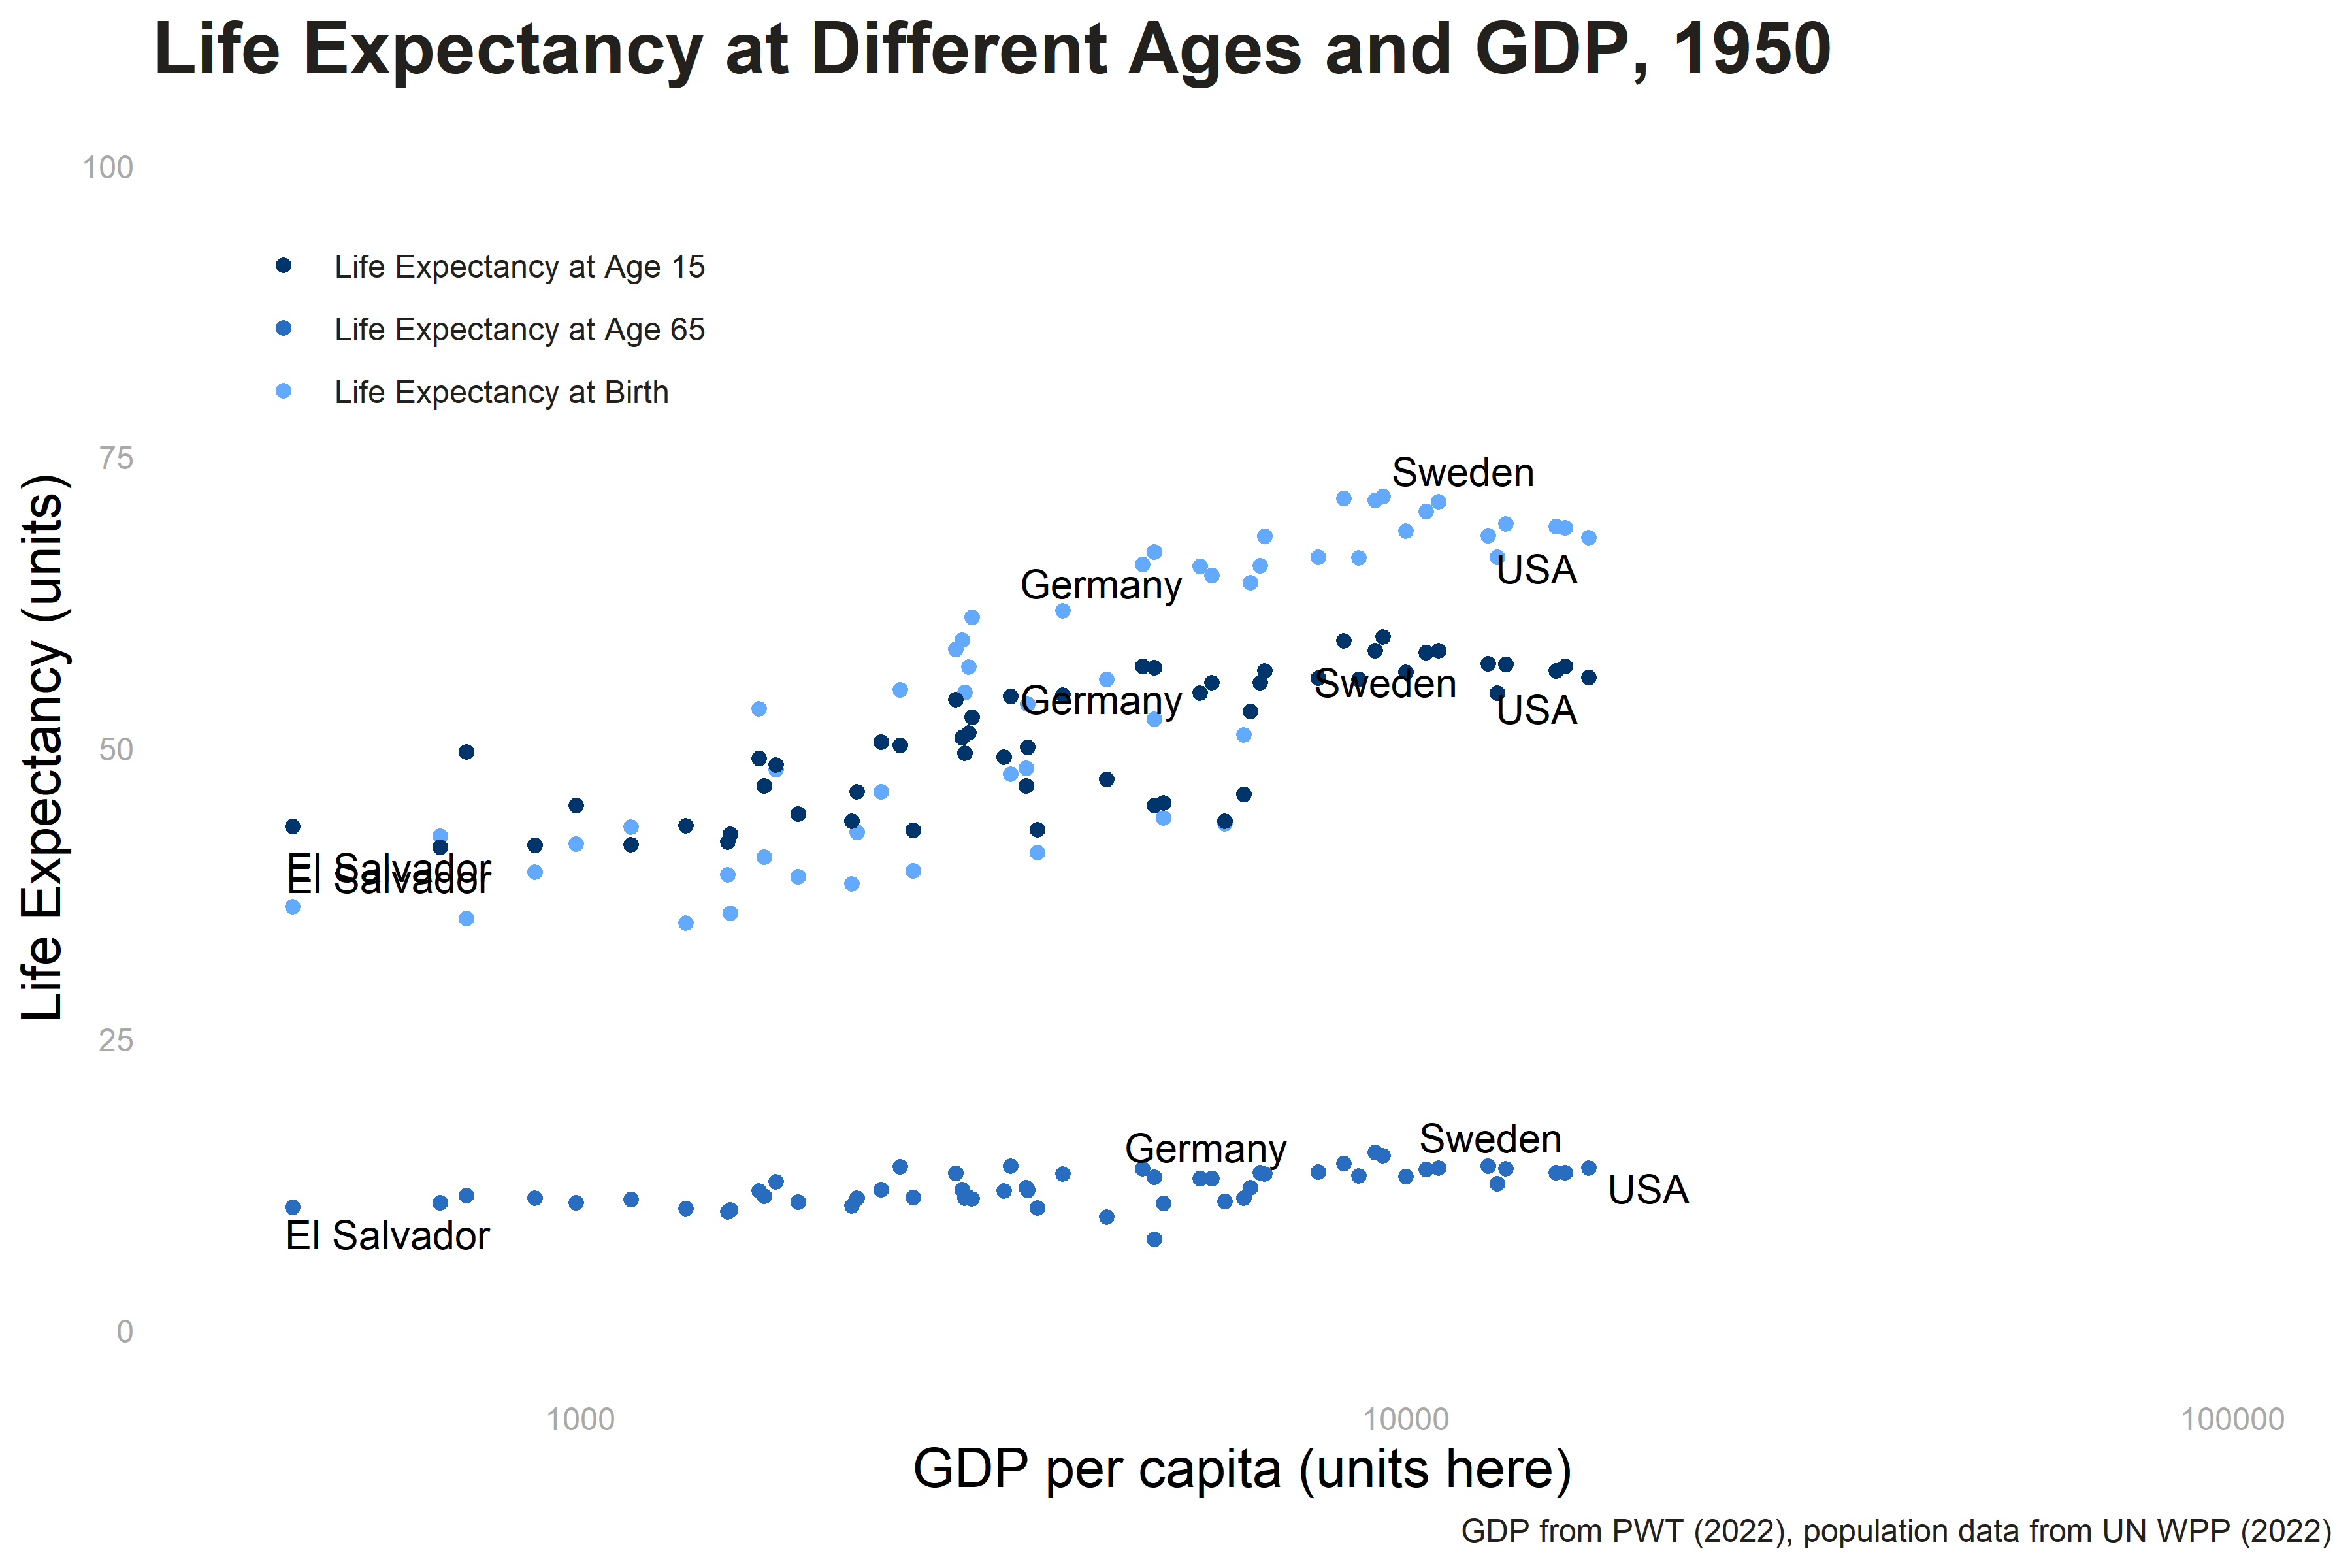
\includegraphics[width=\textwidth]{figures/ECON-412/gdp_pc_le_1950.png}
  \caption{1971}
  \label{fig:sub1}
\end{subfigure}%
\begin{subfigure}[h]{0.5\textwidth}
  \centering
  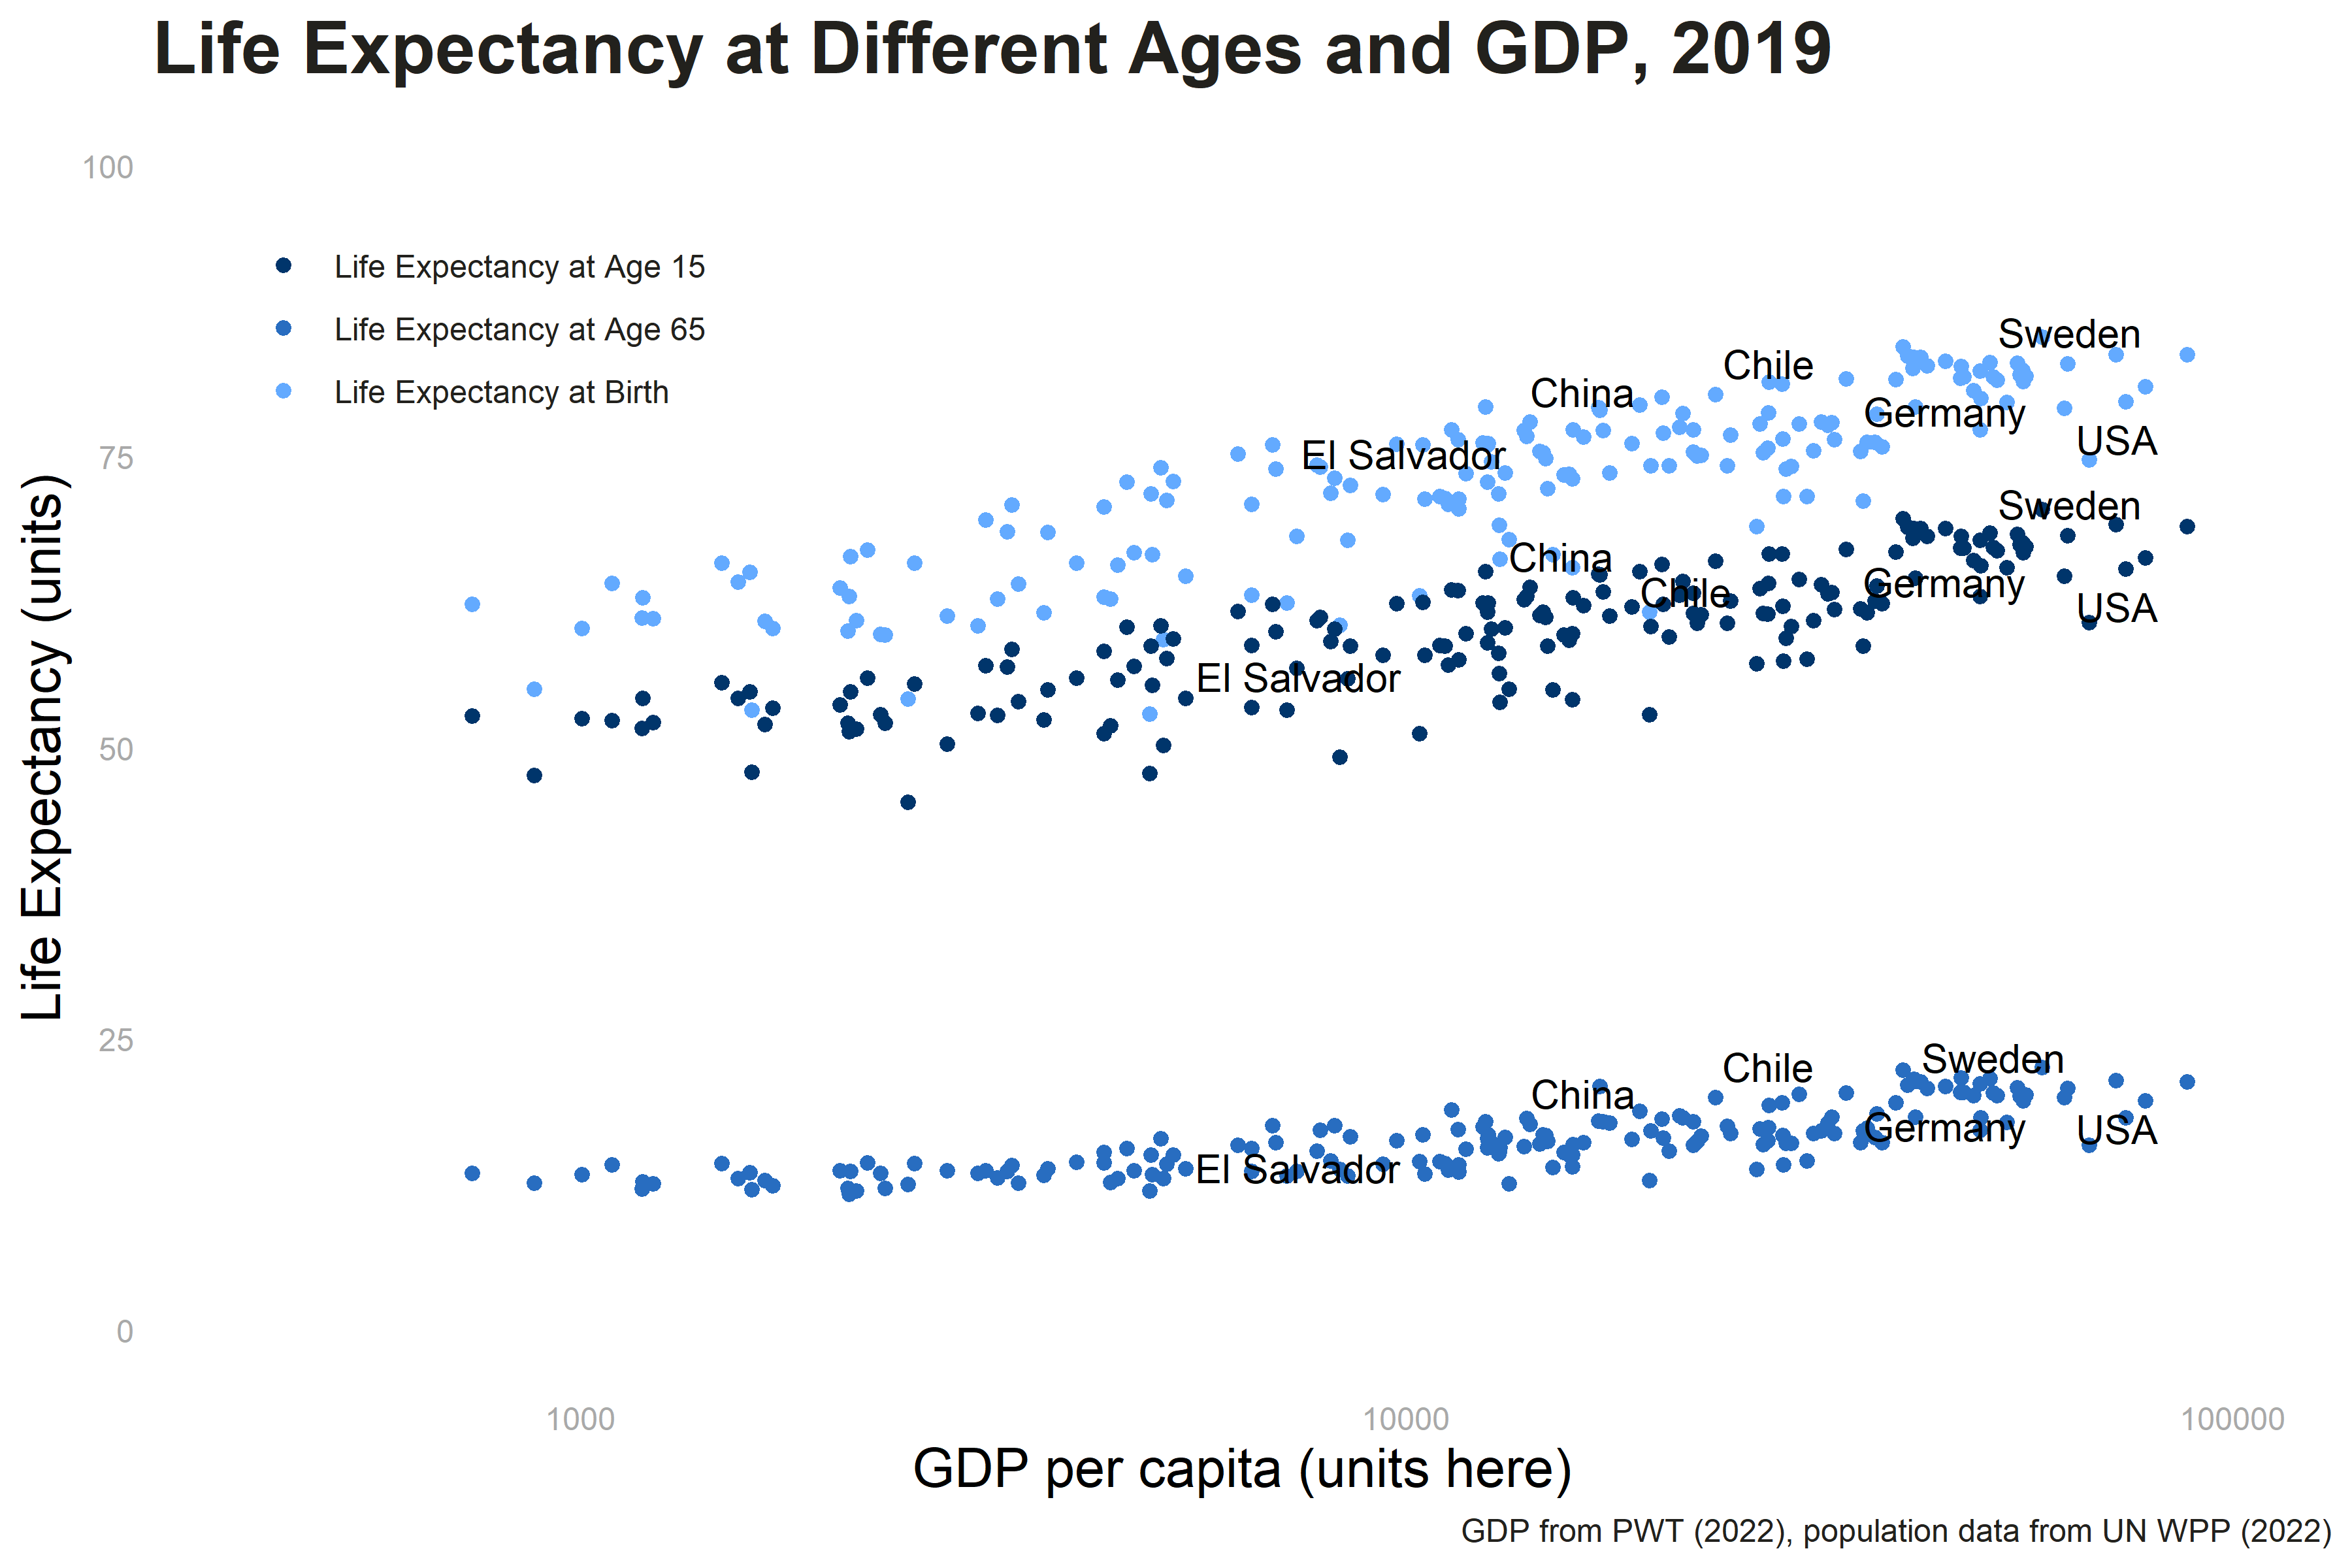
\includegraphics[width=\textwidth]{figures/ECON-412/gdp_pc_le_2019.png}
  \caption{2019}
  \label{fig:sub2}
\end{subfigure}
\caption{Comparison of Life Expectancies to GDP per capita over time}
\label{fig:fig_01}
\end{figure}

\begin{figure}[H]
	\centering % centers
	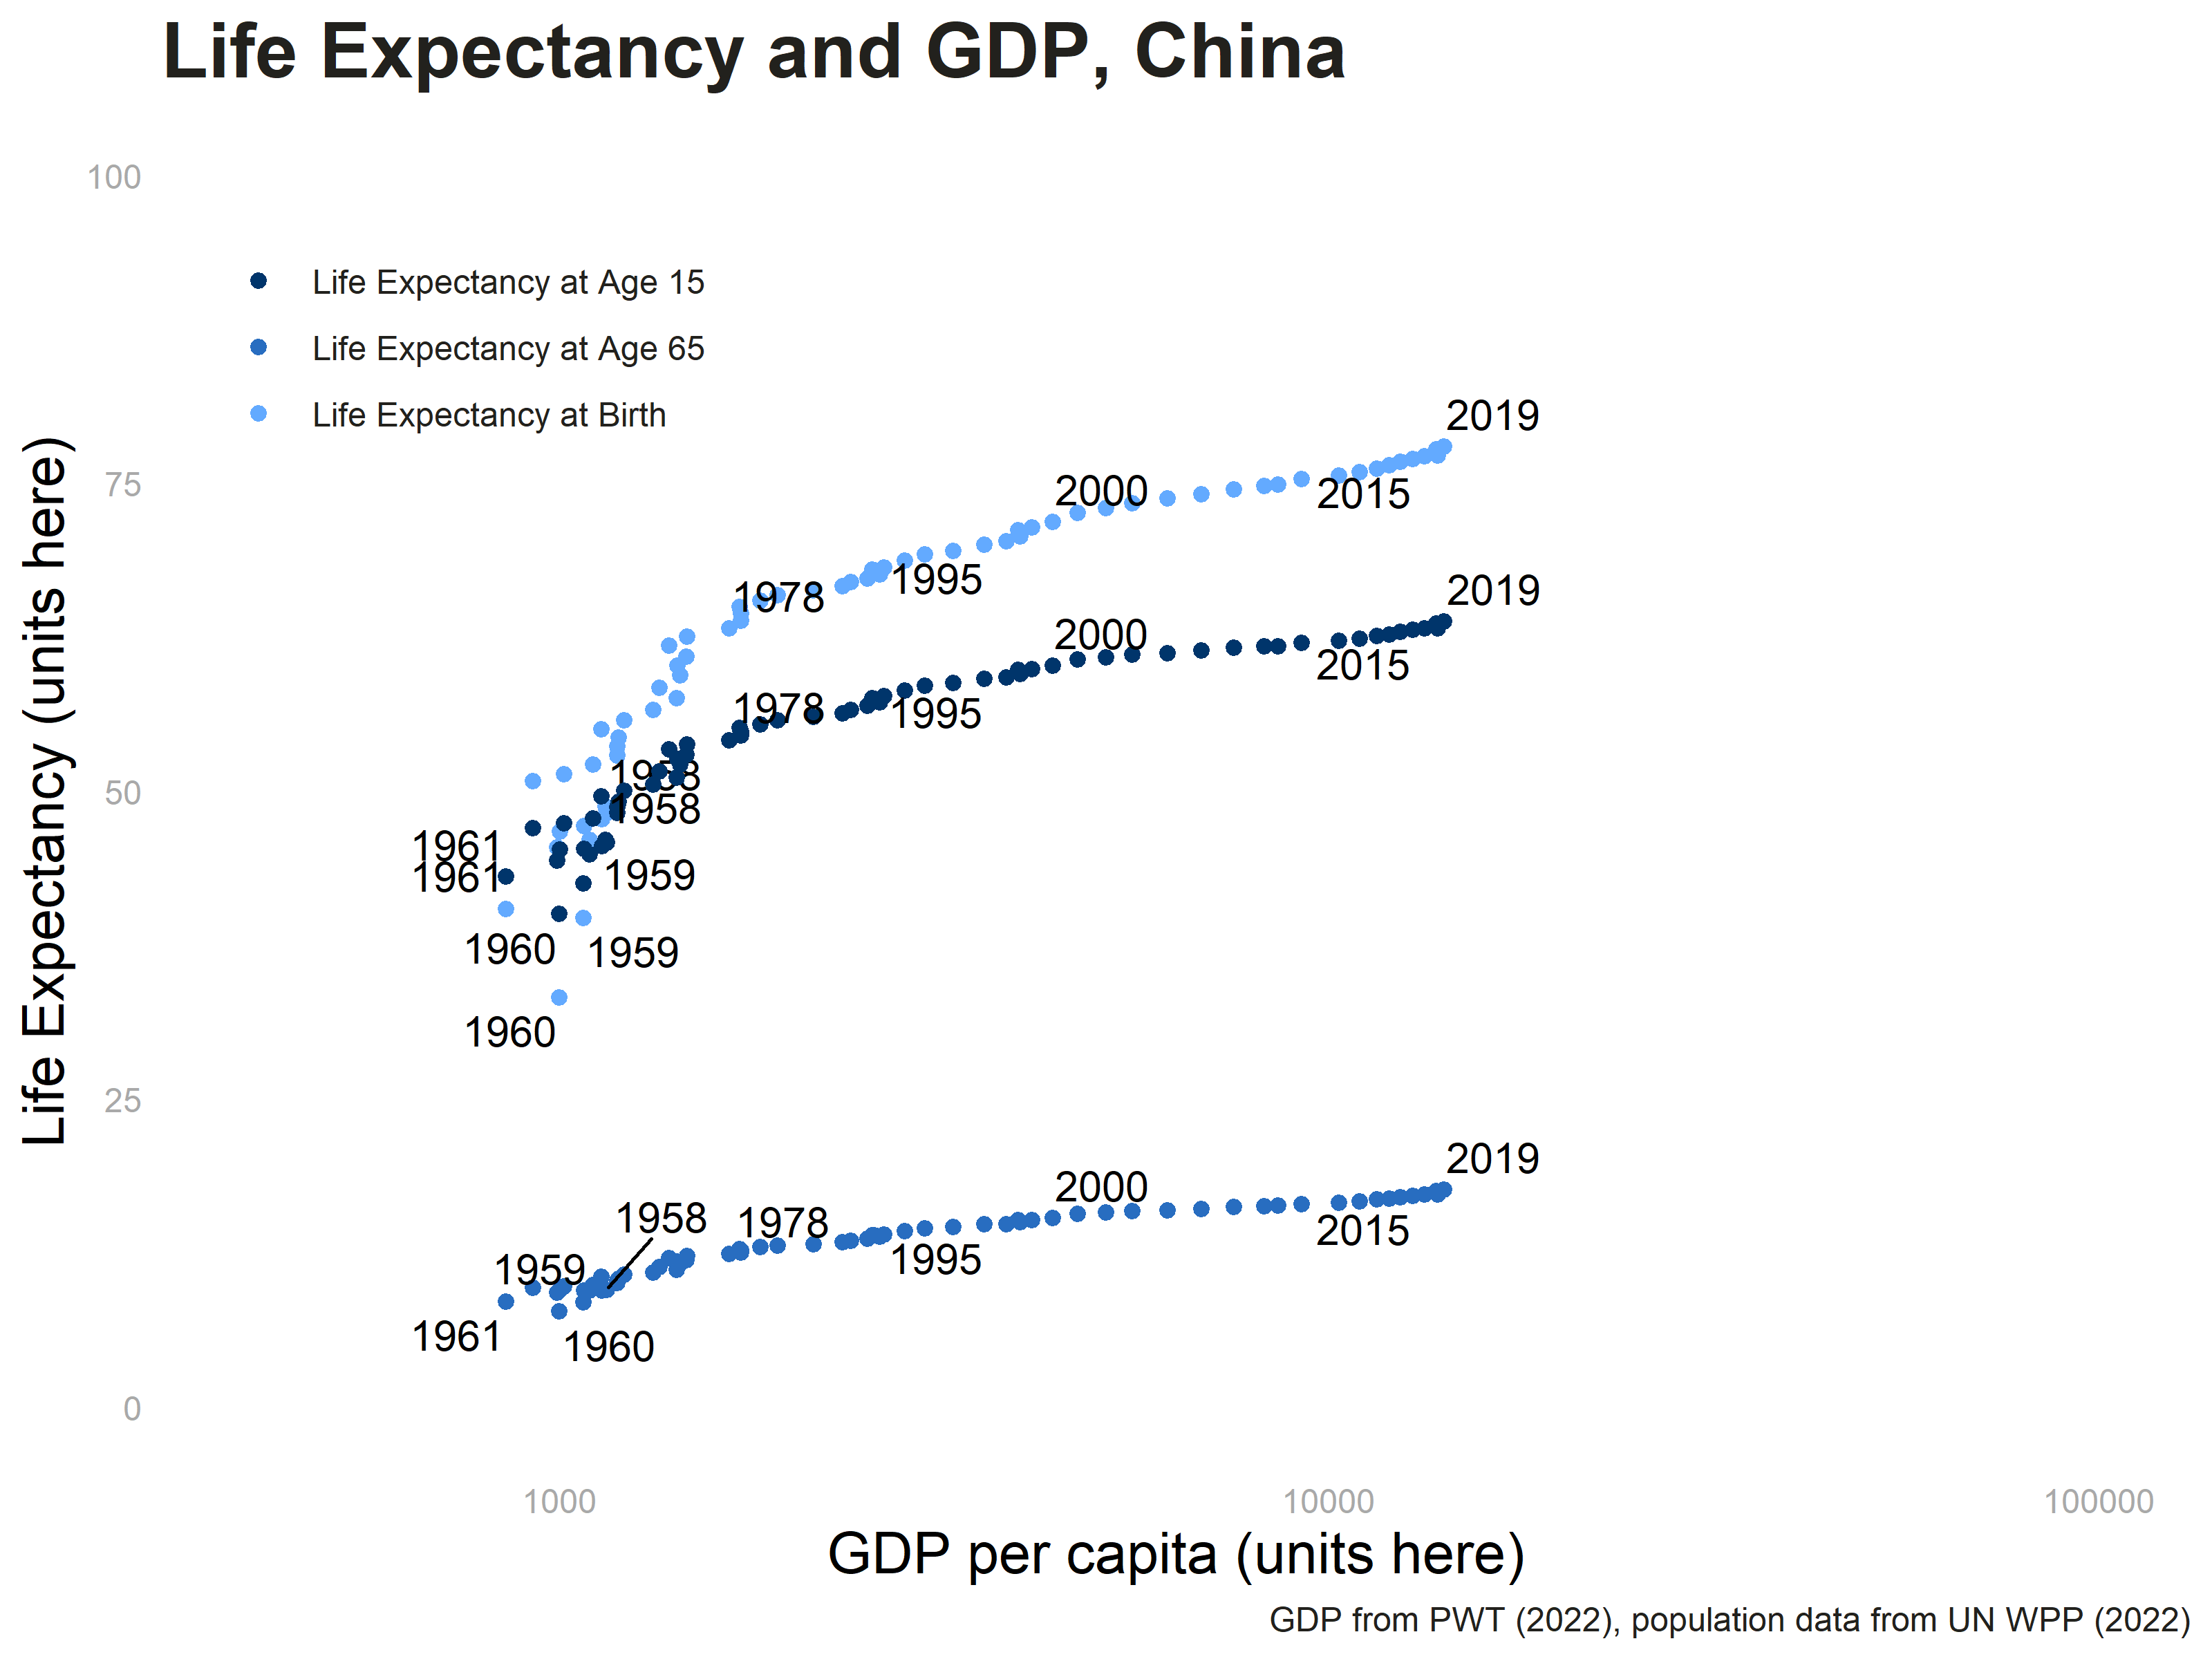
\includegraphics[width=.6\linewidth]{figures/ECON-412/gdp_pc_le_China.png}
	\caption{China's Evolution, 1950-2019} % note caption is required in order to get the cross referencing
	\label{fig:fig3}
\end{figure}



\subsection{Results}

Now let's run some regressions and generate some predictions.


\begin{enumerate}
    \item Adapt your code in \verb+code/03_analysis/03_analysis_hw-03.R+ to generate two tables that correspond to Equations 1 through 5 above. One of these tables should include the results of running regressions from Equations 1 through 3 on the same two years you showed for your figures in Figure~\ref{fig:fig_01}. The code will be similar to that which generated Table~\ref{tab:lecrosssection}. 
    \item The other table should include the results from Equation~\ref{eq:eq_4} and Equation~\ref{eq:eq_5}, with the regression for Equation~\ref{eq:eq_4} restricted to the most recent year, and Equation~\ref{eq:eq_5} a panel over multiple available years. You may find it useful to adapt the code which produced Table~\ref{tab:lepanelregs}.\footnote{It's your choice whether you'd like to restrict the data to a balanced panel, i.e. where all years and all units are available, or whether you'd like to use an unbalanced panel in which you include whatever country-year combinations are available. But whichever you do, spend a couple minutes to think about what the trade-offs are.}
    \item Interpret the results for each column of each table in words (no need to be repetitive, but make clear the distinctions between them). Describe the economic and statistical significance of these coefficients. What is your preferred specification and why? Are any of these results surprising or otherwise noteworthy? 
    \item Adapt the code of \verb+code/04_plots/04_plots_hw-03_template.R+ to generate a scatter plot with GDP per capita on the X axis, and predicted values for greenhouse gas emissions per capita on the Y axis, according to the specification of Equation~\ref{eq:eq_5}. This corresponds fairly closely to the exercise of \citet{grossmanEconomicGrowthEnvironment1995}, yielding a plot like Figure~\ref{fig:fig4}. Do you observe an environmental Kuznets curve? Comment on why or why not. Has your analysis made a causal argument? Comment on why or why not.
\end{enumerate}

\begin{figure}[H]
	\centering % centers
	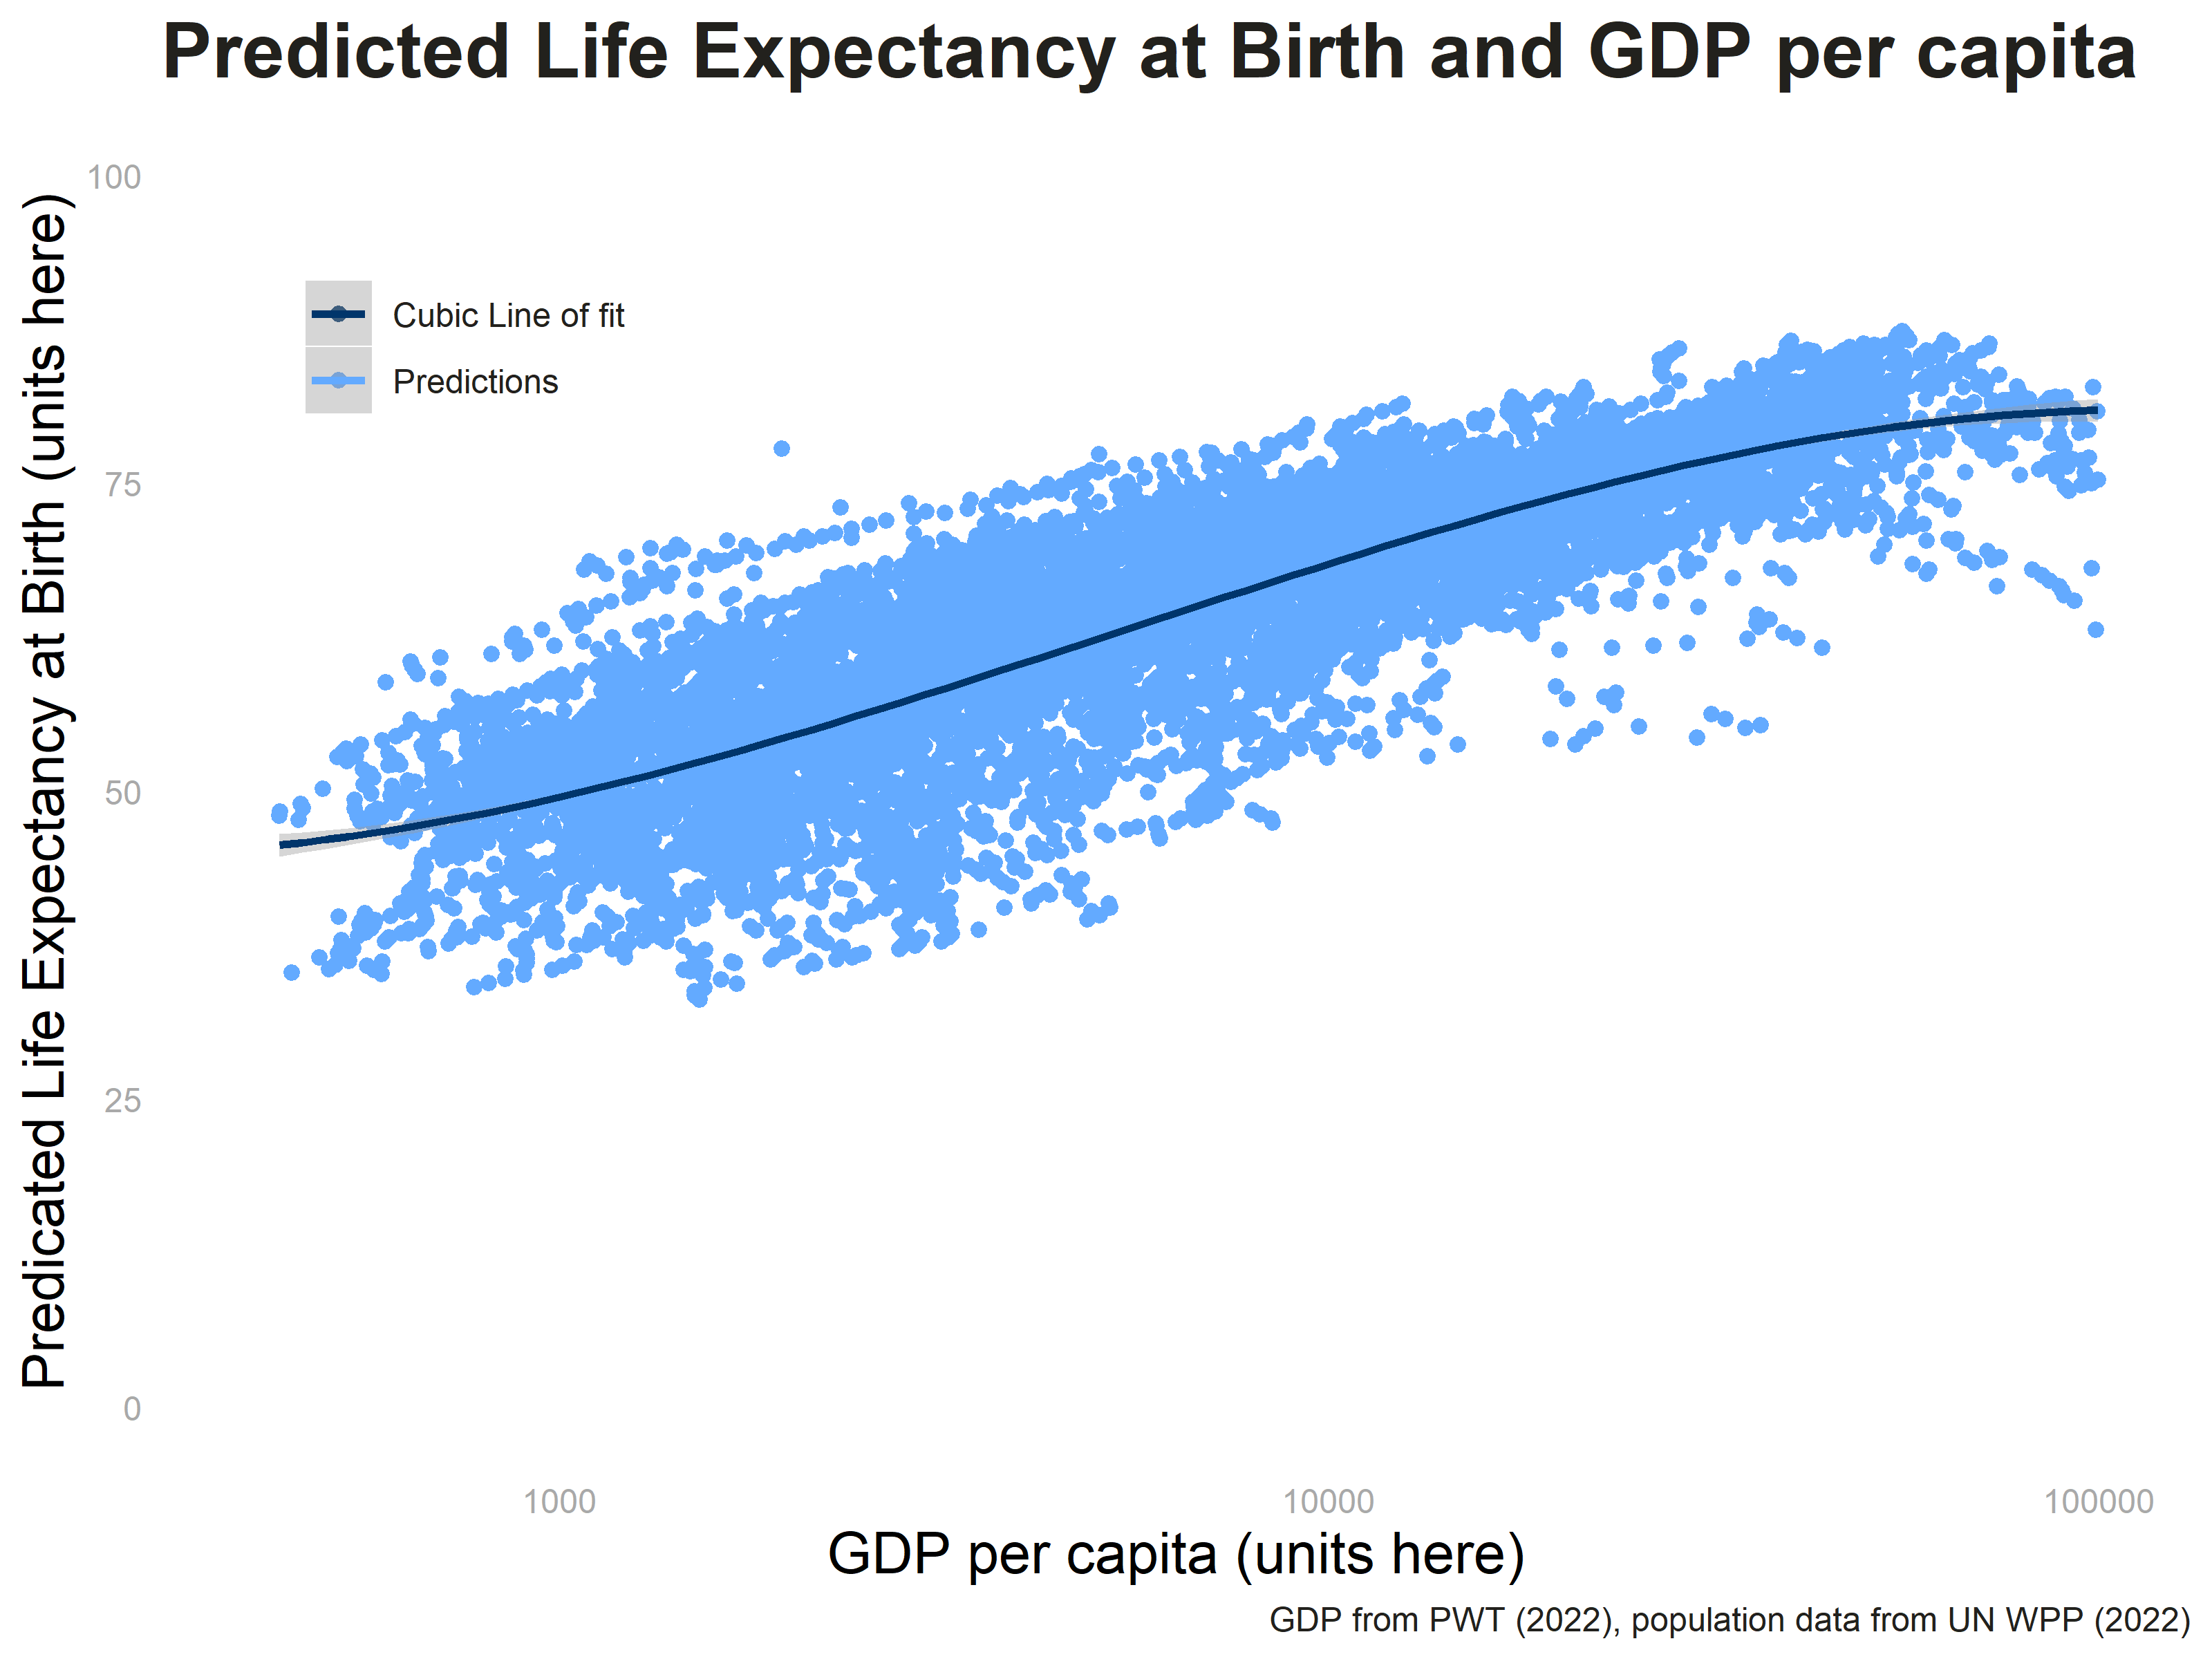
\includegraphics[width=.6\linewidth]{figures/ECON-412/gdp_pc_le_predictions.png}
	\caption{Predicted Values} % note caption is required in order to get the cross referencing
	\label{fig:fig4}
\end{figure}

\begin{comment}

\begin{figure}[H]
	\centering % centers
	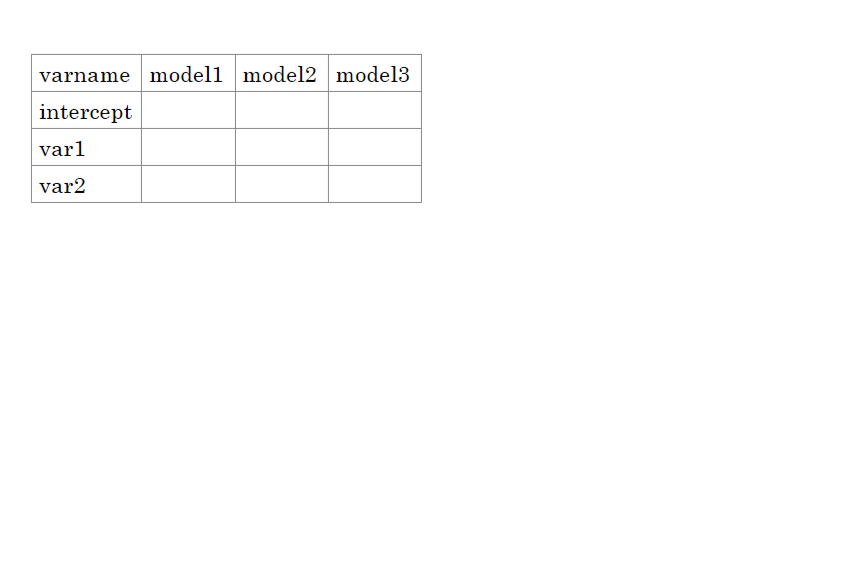
\includegraphics[width=.6\linewidth]{figures/ECON-412/hw-03_table1.png}
	\caption{Example Screenshot for Table Requirement} % note caption is required in order to get the cross referencing
	\label{fig:fig4}
\end{figure}

\end{comment}



% note this requires
%\usepackage{threeparttablex} in the preamble

\begin{table}[H]

\caption{Life Expectancy Cross-Section Comparisons, 1950 and 2019 \label{tab:lecrosssection}}
\centering
\begin{threeparttable}
\begin{tabular}[t]{lcccccc}
\toprule
\multicolumn{1}{c}{ } & \multicolumn{2}{c}{Birth} & \multicolumn{2}{c}{Age 15} & \multicolumn{2}{c}{Age 65} \\
\cmidrule(l{3pt}r{3pt}){2-3} \cmidrule(l{3pt}r{3pt}){4-5} \cmidrule(l{3pt}r{3pt}){6-7}
\multicolumn{1}{c}{ } & \multicolumn{1}{c}{1950} & \multicolumn{1}{c}{2019} & \multicolumn{1}{c}{1950} & \multicolumn{1}{c}{2019} & \multicolumn{1}{c}{1950} & \multicolumn{1}{c}{2019} \\
\cmidrule(l{3pt}r{3pt}){2-2} \cmidrule(l{3pt}r{3pt}){3-3} \cmidrule(l{3pt}r{3pt}){4-4} \cmidrule(l{3pt}r{3pt}){5-5} \cmidrule(l{3pt}r{3pt}){6-6} \cmidrule(l{3pt}r{3pt}){7-7}
  & (1) & (2) & (3) & (4) & (5) & (6)\\
\midrule
Intercept & 42.823 & 67.733 & 42.617 & 42.102 & 11.127 & 14.266\\
 & (1.676) & (0.665) & (6.361) & (4.614) & (0.224) & (0.201)\\
GDP per capita & 0.002 & 0.000 &  &  &  & \\
 & (0.000) & (0.000) &  &  &  & \\
Log GDP per capita &  &  & 2.073 & 2.359 &  & \\
 &  &  & (0.651) & (0.401) &  & \\
TFR &  &  & -1.880 & -1.671 &  & \\
 &  &  & (0.288) & (0.363) &  & \\
GDP (unit) per (unit) &  &  &  &  & 0.213 & 0.093\\
 &  &  &  &  & (0.028) & (0.009)\\
\midrule
Num.Obs. & 55 & 182 & 55 & 182 & 55 & 182\\
Mean & 54.870 & 73.080 & 50.660 & 60.220 & 12.260 & 16.370\\
R2 & 0.611 & 0.508 & 0.769 & 0.724 & 0.360 & 0.572\\
R2 Adj. & 0.604 & 0.505 & 0.760 & 0.721 & 0.348 & 0.569\\
F & 78.666 & 98.508 & 88.414 & 209.054 & 56.186 & 108.220\\
\bottomrule
\end{tabular}
\begin{tablenotes}
\item \textit{Notes: } 
\item Robust standard errors given in parentheses. Population and life expectancy are obtained from \citet{undesaWorldPopulationProspects2022}. Gross domestic product (GDP) is (what units) from \citet{feenstraNextGenerationPenn2015}.
\end{tablenotes}
\end{threeparttable}
\end{table}

\begin{table}[H]

\caption{Panel Regression, Life Expectancy \label{tab:lepanelregs}}
\centering
\begin{threeparttable}
\begin{tabular}[t]{lcccc}
\toprule
\multicolumn{1}{c}{ } & \multicolumn{4}{c}{Life Expectancy at Birth} \\
\cmidrule(l{3pt}r{3pt}){2-5}
\multicolumn{1}{c}{ } & \multicolumn{1}{c}{1950} & \multicolumn{1}{c}{2019} & \multicolumn{1}{c}{Within} & \multicolumn{1}{c}{Twoway} \\
\cmidrule(l{3pt}r{3pt}){2-2} \cmidrule(l{3pt}r{3pt}){3-3} \cmidrule(l{3pt}r{3pt}){4-4} \cmidrule(l{3pt}r{3pt}){5-5}
  & (1) & (2) & (3) & (4)\\
\midrule
Intercept & 33.437 & 62.576 &  & \\
 & (2.405) & (0.789) &  & \\
GDP (units) per (units) capita & 6.714 & 0.891 & 0.821 & -0.141\\
 & (1.609) & (0.082) & (0.065) & (0.048)\\
(GDP(units) per (units))$$^2$$ & -0.373 & -0.014 & -0.008 & 0.001\\
 & (0.217) & (0.002) & (0.001) & (0.000)\\
(GDP (units) per (units))$$^3$$ & 0.006 & 0.000 & 0.000 & 0.000\\
 & (0.008) & (0.000) & (0.000) & (0.000)\\
\midrule
Mean & 54.87 & 73.08 & 64.31 & 64.31\\
Country FE & N & N & Y & Y\\
Time FE & N & N & N & Y\\
Num.Obs. & 55 & 182 & 10201 & 10201\\
R2 & 0.743 & 0.694 & 0.785 & 0.929\\
R2 Within &  &  & 0.302 & 0.035\\
\bottomrule
\end{tabular}
\begin{tablenotes}
\item \textit{Notes: } 
\item Heteroskedascicity-robust standard errors clustered at the country (for within) and country and year (for twoways) levels given in parentheses. Population and life expectancy data are from \citet{undesaWorldPopulationProspects2022}. Gross domestic product (GDP) is (what units) from \citet{feenstraNextGenerationPenn2015}.
\end{tablenotes}
\end{threeparttable}
\end{table}






%\citep{acemogluEnvironmentDirectedTechnical2012} In-text citation with \citet{kummuGriddedGlobalDatasets2018}. \citet{grossmanGrowthTradeInequality2014}
% Front Matter here
\begin{comment}
\maketitle




\begin{abstract}
Your abstract.
\end{abstract}

\tableofcontents % adds a Table of contents
\end{comment}
    


%% Body Templates
    
    %% General Writing Templates
    
\begin{comment}
\section{General Writing Template}


For more see \url{https://www.overleaf.com/learn/latex/Bold,_italics_and_underlining}


These parts are \textbf{emboldened} 
or \underline{underlined} 
and also \textbf{\textit{bold and italicized}}.

You can also italicize with \emph{this command}. The \verb+emph+ and \verb+textit+ behave slightly differently.

\subsection{Common symbols}

If you want to insert an \& or \$ , you need a back slash \ before you do so, since Latex reserves these for alignment commands and math environment commands respectively.



\subsection{IMPORTANT NOTE}
You should never manually type numbers of equations, tables, figures, page numbers, citations, etc. Let Latex handle this referencing and labeling for you.\\

To add a list, use

\begin{enumerate}
    \item This is an item
\end{enumerate}

or 

\begin{itemize}
    \item This is an item
\end{itemize}

For a citation, you typically either want \citet{taylorBuffaloHuntInternational2011} for in-text citations, or at the end of a sentence \citep{taylorBuffaloHuntInternational2011}.
\section{Citations}
- author: Jillian
\subsection{The Basics}
You shouldn't need to manually create a citation style, although you could manually create citations if you didn't feel like using any of the great capabilities of Latex and staring at \verb+@+ signs and trying to figure out where things go.... To each her own.\\

 There are a few packages for if you for some reason needed to input your entries manually, like \verb+biblatex+ or \verb+bibtex+, but you should really be using something like Mendeley, Endnote, or Zotero (if you're a Windows system) or Bibdesk (if Mac). Mendeley, Endnote and Zotero support exporting to a .bib file, so if you're also using Word for inputting citations, you're better off generating and housing your bibliographies in one of those three, and then exporting/syncing to a .bib file that gets sent to your  \verb+Bibliography+ folder. If this is the case, you should never manually edit your \verb+.bib+ file, but only consult to see what automatic citation keys they generated for you. Zotero is something I think is far superior.



 and see somewhere like \url{https://www.overleaf.com/learn/latex/Biblatex_citation_styles}, or, as is more common, use the package \verb+natbib+: 
I want to cite one of the articles from the library:~\cite{acemogluEnvironmentDirectedTechnical2012}. The tilde before that code makes the spacing slightly nicer sometimes.

% see https://www.overleaf.com/learn/latex/natbib_citation_styles for further examples

This document is an example, two items are cited: \textit{The \LaTeX\ Companion} book  - this should have a parentheses around it \citep[see][chap 2]{acemogluEnvironmentDirectedTechnical2012} and Einstein's journal paper \cite{acemogluEnvironmentDirectedTechnical2012}. 

This is a text citation \citet{acemogluEnvironmentDirectedTechnical2012}, parenthetical \citep{acemogluEnvironmentDirectedTechnical2012}, that prints all names of all authors \cite*{acemogluEnvironmentDirectedTechnical2012}, and parenthetical with all authors \citep*{acemogluEnvironmentDirectedTechnical2012}, name only \citeauthor{acemogluEnvironmentDirectedTechnical2012}, and year only \citeyear{acemogluEnvironmentDirectedTechnical2012}. 


For more on natbib styles, see \href{https://www.overleaf.com/learn/latex/Natbib_bibliography_styles}{this page on overleaf}

\subsection{Mendeley, Zotero, Endnote, Jabref ETC with Bibtex}
See the MIT library guide for general info on using all these versions with bibtex: \url{https://libguides.mit.edu/cite-write/bibtex}. MIT has quick guides for all those softwares to get you synced and going quickly.\\

If you're already using one of these primarily, go for it. If you haven't started using a citation software, use one. Just do it.\\

I've done a project in Endnote and ended up not loving it. Lisha uses Zotero. I'm going to try Mendeley next.

The short:\\
\begin{itemize}
\item Zotero can automatically sync with the use of the "Better BibTex" plugin.
\item Mendeley can autosync, but only your entire library
\item Endnote can't autosync
\item Use Jabref if you're on Windows, Latex is your primary compiler, and you can't imagine writing a cited article in Word.
\item Use Bibdesk if the conditions for Jabref hold but you use a Mac.
\end{itemize}

If Mendeley isn't playing nice and generating citation keys, see \url{https://tex.stackexchange.com/questions/461971/mendeley-not-generating-citation-key-on-desktop-version} and see if that fixes it. You shouldn't need to generate your own.

\subsection{Adding a Bib Style (Mac)}
If you're trying to add  a bibstyle on a mac, in the folder ~Library, which you have to make unhidden (google "how to show the Library folder"); and then make folders called \verb+texmf/bibtex/bst+, and dump the .bst file inside there.

Note: there are some installed .bst files, which are what natbib reads to view your citation style, which aren't registering as bib style files. If you want to use them later, drag and drop the .bst into the same folder. 

Those files are currently in\\
\verb+usr/local/texlive/2020/texmf-dist/...+\\
\verb+bibtex/bst/[name of style]/[name of style].bst.+

Note also that you can copy+paste a .bst file from the internet into a new .tex file, but then save as .bst.

\subsection{Actual Citations}
Chances are you'll end up using \verb+natbib+ as the package, so see \url{https://www.overleaf.com/learn/latex/Bibliography_management_with_natbib}. Overleaf recommends using \verb+biblatex+ 
 footnotes


Here I have a footnote\footnote{this is my footnote}
-\section{Cross-Referencing and Hyperlinks}

For more on hyperlinks, note that you need the hyperref package, and then it looks something like this: for more see \href{https://www.overleaf.com/learn/latex/hyperlinks}{this page}.

For more on cross-referencing as regards referring to your tables, see the discussion on cross-referencing in the \verb+basic_tables_template+ in section \ref{table_cross_referencing}.

I've added the package \verb+xurl+ to the preamble. This package was created in 2017 to allow URLs to break across lines (if you have a very long URL and want the entire think to be clickable as a hyperlink). See \url{https://tex.stackexchange.com/questions/3033/forcing-linebreaks-in-url}.
-

 \begin{minipage}{5in} % takes up 5 inches on the LHS of the page
 	\Large Minipage Template \\
 	\large Your name \\
 	\today \\[1.5em] % today's date, then gives a little space below
 \end{minipage}

\end{comment}



    %%% Layout and Formatting


\begin{comment}
\section{Inserting PDF pages directly}

See \url{https://stackoverflow.com/questions/2739159/inserting-a-pdf-file-in-latex}.

You'll need the package in your preamble \verb+pdfpages+. 

The following includes all pages of the pdf:

\includepdf[pages=-,scale=.8,pagecommand={}]{included-pdfs/ECON-511_pset-01_stallman_question-02.pdf}

The following includes pages 1,3 and 5.
\includepdf[pages={1,3,5}]{included-pdfs/ECON-511_pset-01_stallman_question-02.pdf}
% your article style needs to be compatible with chapters
-\chapter{Alice in Wonderland}

\section{The Black Kitten}
  One thing was certain, that the WHITE kitten had had nothing to
do with it:---it was the black kitten's fault entirely.  For the
white kitten had been having its face washed by the old cat for
the last quarter of an hour (and bearing it pretty well,
considering); so you see that it COULDN'T have had any hand in
the mischief.

  The way Dinah washed her children's faces was this:  first she
held the poor thing down by its ear with one paw, and then with
the other paw she rubbed its face all over, the wrong way,
beginning at the nose:  and just now, as I said, she was hard at
work on the white kitten, which was lying quite still and trying
to purr---no doubt feeling that it was all meant for its good.

  But the black kitten had been finished with earlier in the
afternoon, and so, while Alice was sitting curled up in a corner
of the great arm-chair, half talking to herself and half asleep,
the kitten had been having a grand game of romps with the ball of
worsted Alice had been trying to wind up, and had been rolling it
up and down till it had all come undone again; and there it was,
spread over the hearth-rug, all knots and tangles, with the
kitten running after its own tail in the middle.

% This is a sample for Chapter 01
\chapter{Chapter Two or whatever}
\section{The Reproach}

  `Oh, you wicked little thing!' cried Alice, catching up the
kitten, and giving it a little kiss to make it understand that it
was in disgrace.  `Really, Dinah ought to have taught you better
manners!  You OUGHT, Dinah, you know you ought!' she added,
looking reproachfully at the old cat, and speaking in as cross a
voice as she could manage---and then she scrambled back into the
arm-chair, taking the kitten and the worsted with her, and began
winding up the ball again.  But she didn't get on very fast, as
she was talking all the time, sometimes to the kitten, and
sometimes to herself.  Kitty sat very demurely on her knee,
pretending to watch the progress of the winding, and now and then
putting out one paw and gently touching the ball, as if it would
be glad to help, if it might.

  `Do you know what to-morrow is, Kitty?' Alice began.  `You'd
have guessed if you'd been up in the window with me---only Dinah
was making you tidy, so you couldn't.  I was watching the boys
getting in stick for the bonfire---and it wants plenty of
sticks, Kitty!  Only it got so cold, and it snowed so, they had
to leave off.  Never mind, Kitty, we'll go and see the bonfire
to-morrow.'  Here Alice wound two or three turns of the worsted
round the kitten's neck, just to see how it would look:  this led
to a scramble, in which the ball rolled down upon the floor, and
yards and yards of it got unwound again.

  `Do you know, I was so angry, Kitty,' Alice went on as soon as
they were comfortably settled again, `when I saw all the mischief
you had been doing, I was very nearly opening the window, and
putting you out into the snow!  And you'd have deserved it, you
little mischievous darling!  What have you got to say for
yourself?  Now don't interrupt me!' she went on, holding up one
finger.  `I'm going to tell you all your faults.  Number one:
you squeaked twice while Dinah was washing your face this
morning.  Now you can't deny it, Kitty:  I heard you!  What that
you say?' (pretending that the kitten was speaking.)  `Her paw
went into your eye?  Well, that's YOUR fault, for keeping your
eyes open---if you'd shut them tight up, it wouldn't have
happened.  Now don't make any more excuses, but listen!  Number
two:  you pulled Snowdrop away by the tail just as I had put down
the saucer of milk before her!  What, you were thirsty, were you?
 % for use with a report class
\section{Page Formatting}

\subsection{Landscape Format}
See \url{https://tex.stackexchange.com/questions/337/how-to-change-certain-pages-into-landscape-portrait-mode} for the fuller discussion.

If you're compiling with PDFLatex, use the package \verb+pdflscape+. In a normal situation, just add the package \verb+lscape+, and then do like so

\begin{landscape}


\section{A Horizontal Page}

\end{landscape}

\subsection{Adding Vertical Space}
For adding in vertical spacing, use \verb+\vspace{distance}+. 1em is a line, I think.

\subsection{Centering}
Then \verb+\centering+ says to center, and best with beginning and ending curly brackets around the text desired to be centered. It will center everything within its "environment", which can mean the entire following document, so you can put it in a "minipage" environment, which will limit the centering to just that block of text you designate as your minipage.

For more on minipage see \url{https://www.sascha-frank.com/latex-minipage.html}

\noindent
\begin{minipage}{\textwidth} % establishes a different environment
\centering
\vspace{1em}
[Figure 2 about here]
\vspace{1em}

\end{minipage}

\noindent
Here is some more text. Notice it is no longer centered.\\


Alternatively, you can use \verb+\begin{center}+ as well. 

\begin{center}
\vspace{1em}
This text is centered now.
\vspace{1em}
\end{center}

\noindent
This text is back to normal. 
 % for things like landscape pages
-
\chapter{Introduction}

\section{SECTION 1}
The text for Section 1 goes here, without brackets.

\section{SECTION 2}
Section 2 text.

\subsection{Subsection heading goes here}

Subsection 1 text

\subsubsection{Subsubsection 1 heading goes here}
Subsubsection 1 text

\subsubsection{Subsubsection 2 heading goes here}
Subsubsection 2 text

\section{SECTION 3}
Section 3 text. The dielectric constant at the air-metal interface
determines the resonance shift as absorption or capture occurs.

 % for adding sections, subsections, subsubsections
\section{Creating Theorems, Hypotheses, and Lemmas}\label{theorems-hypotheses}

If you'd like to have something titled to which you can refer, like hypotheses 1-4, theorems, definitions, assumptions and so forth, you can create a command in the preamble that defines this new environment. 

For an intro tutorial, see \url{https://www.overleaf.com/learn/latex/theorems_and_proofs}, which has most of what you should need. Many examples below have been taken from here.

See \url{https://tex.stackexchange.com/questions/386905/hypothesis-with-amsthm-package}. You need \verb+amsthm+, and then check this preamble (the one in \verb+main-article+) in the area under the \verb+amsthm+ package. The high level of customization uses \verb+thmtools+, and the \verb+\cref+ uses the \verb+cleverref+ package, a package for fancy cross references. 

Note, though, that \verb+cleverref+ can clash with the \verb+cases+ package: \url{https://tex.stackexchange.com/questions/201437/cleveref-and-cases-packages-clash}. 

See \url{https://tex.stackexchange.com/questions/36295/cross-reference-packages-which-to-use-which-conflict} for tons of pros and cons you'll hopefully never need. 

The short: \verb+cleverref+ is a great package. Just make sure that \verb+cleverref+ is the last loaded cross-referencing package (the last one in your preamble)

Note also that the "hypothesis" environment used \verb+amsthm+, and the fancy cross referencing used \verb+cleverref+. You wouldn't need \verb+cleverref+ just to introduce the hypothesis environment, although it did require \verb+thmtools+ to make it so customized.

 \begin{hyp}[Test hypothesis] \label{hyp:a}This is my first hypothesis. \end{hyp}
 \begin{hyp} \label{hyp:b}This is my second hypothesis. \end{hyp}

  \Cref{hyp:a,hyp:b}.

Additionally, you can use the easier redefinition of commands from \verb+amsthm+ to designate theorems and lemmas that go under theorems, for instance:



\section{Examples}

\begin{theorem}[Test theorem]
This is the first theorem
\end{theorem}

\begin{corollary}
Here's a corollary to the theorem
\end{corollary}




\begin{theorem}
Let $f$ be a function whose derivative exists in every point, then $f$ is 
a continuous function.
\end{theorem}

\begin{theorem}[Pythagorean theorem]
\label{pythagorean}
This is a theorema about right triangles and can be summarised in the next 
equation 
\[ x^2 + y^2 = z^2 \]
\end{theorem}

And a consequence of theorem \ref{pythagorean} is the statement in the next 
corollary.

\begin{corollary}
There's no right rectangle whose sides measure 3cm, 4cm, and 6cm.
\end{corollary}

You can reference theorems such as \ref{pythagorean} when a label is assigned.

\begin{lemma}
Given two line segments whose lengths are $a$ and $b$ respectively there is a 
real number $r$ such that $b=ra$.
\end{lemma}

\begin{assumption}
I am making an assumption
\end{assumption}

\section{Restarting the examples}

\begin{theorem}
Let $f$ be a function whose derivative exists in every point, then $f$ is 
a continuous function.
\end{theorem}

You can reference theorems such as \ref{pythagorean} when a label is assigned.

\begin{lemma}
Given two line segments whose lengths are $a$ and $b$ respectively there is a 
real number $r$ such that $b=ra$.
\end{lemma} % for customizing so that you can label and cross-reference your hypotheses, theorems, and so on

\section{Alternatively}

We can also use the \verb+answers+ package.

\section*{Problem 1}
 Suppose that the cost function for mitigation is $C=40A^2$ and that the benefits are given by $B=800A-10A^2$, where $A$ gives tons of mitigation. Assume every ton of pollution causes harm.
 \Opensolutionfile{ans}[ans1] % starts running the solution file
\begin{ex}
What level of mitigation minimizes total abatement costs?

\begin{sol}
  As the cost function is increasing everywhere there's positive mitigation, total abatement costs are only minimized when there's no abatement, i.e. $A=0$
\end{sol}
  \end{ex}
  
       \begin{figure}[H]
	\centering % centers
	\includegraphics[width=.8\linewidth]{figures/frog.jpg}
	\caption{Phase Diagram} % note caption is required in order to get the cross referencing
	\label{fig:ps02phasediag}
\end{figure}


\Closesolutionfile{ans}

\section{Answers}
\input{ans1}

\end{comment}



    %%% Math Templates

\begin{comment}


\section{Math Equations}



\subsection{Equations}
The following is adapted from \url{https://www.overleaf.com/learn/latex/mathematical_expressions}.



Equations in-line can be demarcated like so \(x^2 + 2^e = \pi \) or $42=2a-i$.

This basic math environment centers equations on a single line:

\[ \cos(2\pi)+\sinh(x)=\lim_{n\to \infty} f^n(\cdot)\]

Number equations with the \verb+equation+ environment. To use this environment, you need the package \verb+amsmath+, but if you're using Latex you probably want this package anyways.

\begin{equation}
	\int_{0}^{\infty} [\sqrt{n}+4] dx + \sum_{i=1}^{-\infty} A_{jkl}^{3}
\end{equation}

See \url{https://www.overleaf.com/learn/latex/Aligning%20equations%20with%20amsmath} for explanations\\

For more operators and functions, see \url{https://www.overleaf.com/learn/latex/Operators}.\\

\subsubsection{Split and a fraction}
If you have several lines of equations but you're really only interested in one equation, you can group them together into a single equation. Note that the \& is setting the delimiter. This is common (tables and matrices also use this delimiter).\\

This is also how you do fractions. Fractions can nest within fractions.

\begin{equation} \label{eq1}
	\begin{split}
		A & = \frac{\pi r^2}{2} \\
		& \neq  \frac{1}{2\frac{2\alpha}{48}} \pi r^2\\
		B & = \frac{2\{A,b,c\}}{\varepsilon}\\
		\mathbb{R} & \supset [0,1]
	\end{split}
\end{equation}

\subsubsection{Cross-Referencing Equations}
You can also reference equations by giving them a label. 
This \verb+\ref+ is a command in the Latex kernel. Note that it doesn't put parentheses around the number.

\begin{equation} \label{eu_eqn}
	e^{\pi i} + 1 = 0
\end{equation}

The beautiful equation \ref{eu_eqn} is known as the Euler equation


The other way to do it, \verb+\eqref+, uses \verb+amsmath+.
\begin{equation} \label{eq:anothereq}
	\varnothing = \emptyset
\end{equation}

See \url{https://tex.stackexchange.com/questions/107422/what-is-the-difference-between-eqref-and-ref}.


The varnothing in equation \eqref{eq:anothereq} requires the package \verb+amssymb+.


\subsubsection{Labeling or not}
If you want just a specific equation labeled within your align environment, you can either force a tag or force no tag. the \verb+\notag+ command can go at the beginning or end of the equation, it just has to be on the correct line.\\

Since \verb+align+ automatically labels each equation, you can pick out a particular equation and refer to it: 

\begin{align} 
	2x - 5y 		&=  8 \label{eq:a}\\ 
	3x + 9y 		&=   -12 \notag \\
	\notag  \Psi 	&=  \emptyset  \\
\end{align}

The first equation above is equation \eqref{eq:a}

\subsubsection{Aligning Equations}
If you're doing a row of equations and specifically want to align them, put them in the align environment. The asterisk in \verb+\begin{align*}+ and \verb+\end{align*}+ says "don't label this equation" Note the double backslash to put on a new line, and note that you need the asterisk both at the beginning and the end of  environment.

\begin{align*} 
	2x - 5y &=  8 \\ 
	3x + 9y &=  -12
\end{align*}

Another example:

\begin{align*}
	x&=y           &  w &=z              &  a&=b+c\\
	2x&=-y         &  3w&=\frac{1}{2}z   &  a&=b\\
	-4 + 5x&=2+y   &  w+2&=-1+w          &  ab&=cb
\end{align*}

Hopefully you'd have found a nicer way to type that up. All the ampersands take a while to figure out.

\subsubsection{... or not}
Or if you don't want to align anything: 

\begin{gather*} 
	2x - 5y =  8 \\ 
	3x^2 + 9y =  3a + c
\end{gather*}





\subsection{Bracketing}

You can tell latex to decide how big the brackets should be in an equation:

\[ 
F = G \left( \frac{m_1 m_2}{r^2} \right)
\]

 \[ 
\left[  \frac{ N } { \left( \frac{L}{p} \right)  - (m+n) }  \right]
\]


You need to have both left and right in order for the parentheses to register. If you don't want one of them, replace with a dot that makes the brace invisible.


 This is a common mistake that leads to compiling errors.
 \begin{equation}
 \begin{split}
 y  = 1 + & \left(  \frac{1}{x} + \frac{1}{x^2} + \frac{1}{x^3} + \ldots \right. \\
 & \quad \left. + \frac{1}{x^{n-1}} + \frac{1}{x^n} \right)
 \end{split}
 \end{equation}


 \subsubsection{Types of Brackets and Some Symbols}
 
 \begin{align}
	& (a+b) 							& \leq  4\\
 	& [x+y] 							& \neq  3\\
 	& \{ z+f\} 							& \subsetneq \beta\\
 	& \langle \vec{x} + \hat{y} \rangle & \subseteq \tilde{z}\\
 	& | \overline{X}_n - \mu | 			& \approx \frac{1}{n}\sum_{i=1}^{n} X_i \\
 	& \| \Theta - \chi^2 \| 			& \geq 42
 \end{align}

\subsection{Theorems, Assumptions, and Hypotheses}
 See the section on \verb+theorems-hypotheses-template+ in \verb+02_layout-formatting+ for how to add theorems and hypotheses and such to the environment, in \ref{theorems-hypotheses}. For the quick, see \url{https://www.overleaf.com/learn/latex/theorems_and_proofs}.
  % equations formatting, how to align equations, how to tag and label equations
\section{Math}
If you want all the great math symbols, see \url{https://oeis.org/wiki/List_of_LaTeX_mathematical_symbols}. If you can't find something in there, check out \url{http://tug.ctan.org/info/symbols/comprehensive/symbols-a4.pdf}.

For a pretty empty set, put \verb+\usepackage{amssymb}+ in your preamble, and use $\varnothing$ rather than $\emptyset$ or $\{\}$.


For script characters, use \verb+\mathcal{P}+ for, for instance, $\mathcal{F}$. \\

Note that there are two epsilons, \verb+epsilon+ ($\epsilon$) and \verb+varepsilon+ ($\varepsilon$)

 % common math symbols and where to look for all the symbols you might want
\begin{comment}
\section{Math: Matrices}

Adapted from \url{https://www.overleaf.com/learn/latex/Matrices}


See also the documentation for the \verb+mathtools+ package for \verb+psmallmatrix+ and \verb+bsmallmatrix+ and more.

All the matrices you might want. Note that \verb+\\+ is the newline command, and \verb+&+ is the alignment operator.

\begin{equation*}
\begin{matrix}
	1 & 2 & 3\\
	a & b & c
\end{matrix}
\end{equation*}

\begin{equation*}
\begin{pmatrix}
	1 & 2 & 3\\
	a & b & c
\end{pmatrix}
\end{equation*}

\begin{equation*}
\begin{bmatrix}
	1 & 2 & 3\\
	a & b & c
\end{bmatrix}
\end{equation*}

\begin{equation*}
\begin{Bmatrix}
	1 & 2 & 3\\
	a & b & c
\end{Bmatrix}
\end{equation*}

\begin{equation*}
\begin{vmatrix}
	1 & 2 & 3\\
	a & b & c
\end{vmatrix}
\end{equation*}

\begin{equation*}
\begin{Vmatrix}
	1 & 2 & 3\\
	a & b & c
\end{Vmatrix}
\end{equation*}


For funkier matrices, you can make the brackets manually:


\begin{equation*}
\left\lceil
\begin{matrix}
	1 & 2 & 3\\
	a & b & c
\end{matrix}
\right\rceil
\end{equation*}

\begin{equation*}
\left\langle
\begin{matrix}
	1 & 2 & 3\\
	a & b & c
\end{matrix}
\right\rangle
\end{equation*}

\subsection{Inline Matrices}

Trying to typeset an inline matrix here
$\begin{pmatrix}
	a & b\\ 
	c & d
\end{pmatrix}$ 
but it looks too big, so let's try 
$\big(\begin{smallmatrix}
	a & b\\
	c & d
\end{smallmatrix}\big)$ 
instead.
\end{comment}


\section{Writing an Arbitrary System of Equations in Matrix Form}

Let $X_{ij}$ denote the $i$th regressor for the $j$th observation, for $i=1,\ldots,k$ and $j=1,\ldots,n$
        \begin{equation*}
            \begin{bmatrix}
Y_1 \\ Y_2 \\ \vdots \\ Y_n
\end{bmatrix} =
\begin{bmatrix}
\beta_0 + \beta_1 X_{11} + \beta_2 X_{21} + \ldots + \beta_kX_{k1}\\
\beta_0 + \beta_1 X_{12} + \beta_2 X_{22} + \ldots + \beta_kX_{k2}\\
\ldots\\
\beta_0 + \beta_1 X_{1n} + \beta_2 X_{2n} + \ldots + \beta_kX_{kn}
\end{bmatrix}+
\begin{bmatrix}
\varepsilon_1 \\
\varepsilon_2 \\
\vdots\\
\varepsilon_n
\end{bmatrix}
        \end{equation*}

We can separate the regressors and coefficients as
\begin{equation*}
            \begin{bmatrix}
Y_1 \\ Y_2 \\ \vdots \\ Y_n
\end{bmatrix} =
\begin{bmatrix}
1 & X_{11} & X_{21} & \ldots & X_{k1}\\
1 & X_{12} & X_{22} & \ldots & X_{k2}\\
\vdots & \vdots & \vdots & \vdots & \vdots \\
1 & X_{1m} & X_{2n} & \ldots & X_{kn}\\
\end{bmatrix}
\begin{bmatrix}
\beta_0 \\
\beta_1 \\
\vdots\\
\beta_n
\end{bmatrix}+
\begin{bmatrix}
\varepsilon_1 \\
\varepsilon_2 \\
\vdots\\
\varepsilon_n
\end{bmatrix}
\end{equation*}
Then $\beta = (X'X)^{-1}X'Y$


 % basic matrices format
\end{comment}




    %%% Tables and Figures
    
\begin{comment}
% For general placement of graphics
\section{Placing Graphics where you want them}

See \url{https://www.overleaf.com/learn/latex/Positioning_images_and_tables}. To be finished later. 

\end{comment}





        % Figure Templates

\begin{comment}
% this is a very basic figure insertion. You can have subfigures or basically whatever you can think of.
%[H] forces it to be HERE. otherwise latex will put it at the next convenient place


\begin{figure}[H]
	\centering % centers
	\includegraphics[width=.6\linewidth]{frog.jpg}
	\caption{Here's my caption} % note caption is required in order to get the cross referencing
	\label{fig:frog}
\end{figure}

\begin{figure}[H]  %for putting in a single figure
\centering
\includegraphics[width=.7\linewidth]{figures/pv/sekhon_net-structure.jpg}\\
\tiny{Source: Jas Sekhon's Lecture Notes}
\end{figure}

This refers to the \textbf{ figure} above, Figure\ref{fig:frog}.

%This has some text that has been \textit{italicized.}
\end{comment}





        % Table Templates
        



\begin{comment}
\subsection{Tables with Stata's Estout Output}

% requires commands for the estauto, search in the preamble


\begin{singlespace}
\begin{table}[!htbp]
\caption{Summary Statistics for PM 2.5 by Sensor Location in Minnesota} \label{tab:city-sum-stats}
\begin{center}

%% estauto	  
	  \estauto{tables/tables-from-stata/table-city-pm25-mean}{10}{c}

\begin{minipage}{0.7\textwidth}
\small{\textit{Note}: Readings taken for available data as daily averages from January 01, 2016 to December 31, 2018. Levels of 0-12 are considered good (corresponding to an AQI of 0-50), 12.1-35.4 are moderate (AQI 51-100); 35.5-55.4 unhealthy for sensitive groups (AQI 101-150); and 55.5-150.4 unhealthy (AQI 151-200). Data from the Minnesota Pollution Control Agency}
\end{minipage}	  

\end{center}
\end{table}
\end{singlespace}




\section{Fancier Tables: Threeparttable}
Making highly editable tables can be a bit of a hassle. To have a table with notes, you'll probably want the package \verb+threepartable+. For a table that spans multiple pages, you need \verb+longtable+. For a table that spans multiple pages AND has customizable notes, you'll want to add the package \verb+threeparttablex+, which allows you to use \verb+longtable+ with \verb+threeparttable+, but note that you'll need to spend a little time finagling with the table notes in order to get this to work. See \verb+longtable-with-text-wrapping+ for longtable examples.

(to be continued)
\subsection{threeparttable}
See \href{https://tug.org/pracjourn/2007-2/asknelly/}{here} for some examples.
The following is an example from \href{https://tex.stackexchange.com/questions/118743/threeparttable-notes-layout}{tex stack exchange}


\begin{table}[htp]
\caption{Some very informative caption}
\begin{center}
\begin{threeparttable}
\begin{tabular}{c c c c}
    \toprule
    \textbf{1st Column} & \textbf{2nd Colimn} & \textbf{3rd Colimn} & \textbf{4th Colimn} \\ \midrule
      QWERTY\tnote{1}   &                     &                     &  \\
      ASDFGH\tnote{2}   &                     &                     &  \\ \bottomrule
\end{tabular}
\begin{tablenotes}
\item[1] qwerty; \item[2] asdfgh
\end{tablenotes}
\end{threeparttable}
\end{center}
\label{table:simDisimCoefNewDef}
\end{table}



\begin{table}[H]
\centering
\caption{...}
\footnotesize
{
\def\sym#1{\ifmmode^{#1}\else\(^{#1}\)\fi}
\begin{threeparttable}

\begin{tabular}{c c c c}
    \toprule
    \textbf{1st Column} & \textbf{2nd Colimn} & \textbf{3rd Colimn}\tnote{\dag} & \textbf{4th Colimn} \\ \midrule
      QWERTY\tnote{1}   &                     &                     &  \\
      ASDFGH\tnote{2}   &                     &                     &  \\ \bottomrule
\end{tabular}
  \begin{tablenotes}
    \item[$*$] $p<0.1$, \sym{**} $p<0.05$, \sym{***} $p<0.01$
    \item[\dag] These ... \smallskip
    \item \emph{Note:} This is a note. I'm not sure if it will switch onto the next line as I'd like, so here I am going to go ahead and keep writing to see if it will indeed switch lines
  \end{tablenotes}

\end{threeparttable}
}
\label{tbl:name}
\end{table}



   
\section{Tables}\label{tables_basics}

See \url{https://www.overleaf.com/learn/latex/tables} for the basics.


For some best practices on sending tables to Latex, see the \href{https://blogs.worldbank.org/impactevaluations/nice-and-fast-tables-stata}{World Bank Blog Post here}. In particular, see \href{http://www2.stat.duke.edu/~rcs46/lectures_2015/01-markdown-git/slides/naming-slides/naming-slides.pdf}{these slides} on how to name your files.


See \url{https://tex.stackexchange.com/questions/12672/which-tabular-packages-do-which-tasks-and-which-packages-conflict} for more information on table packages. There are a lot of packages that do table-like things, and oftentimes which ones you use will depend on what the default output (Stata, R, Matlab) uses when it's outputting.\\

See especially that discussion if you find yourself needing tables that span pages, get really long, get really wide, or need captioning.\\

Must-have packages for the academic: \verb+booktabs+, \verb+array+, \verb+tabularx+, \verb+threeparttable+. The first is good for customization and professional-looking tables. The second is general customization and shows up in all sorts of funky places. The third similarly, and the fourth for making tweaks as well. Another common one is \verb+multirow+

If you're sending tables from a statistical package like R or Stata to Latex, DO NOT edit them manually in Latex. Figure out your commands for the statistical package (like outreg for stata) and do all your editing at the script level in the statistical software. Then, you should send the tables to the subfolder "Tables" in whatever directory houses your master latex file, and you can use \verb+\input{Tables/yourtablename.tex}+ to tell Latex to use the table file. 

For compatibility with Stata, see for example the documentation for \verb+outreg2+ at \url{http://repec.org/bocode/o/outreg2.html}. Commands like \verb+estout/esttab+ will get you results quickly, but aren't very customizable. See for example Luke Stein's discussion \href{https://lukestein.github.io/stata-latex-workflows/}{here}. For a higher-cost but beautiful setup, see \verb+tabout+, whose documentation has a bunch of beautiful examples and Stata do files at \href{http://ianwatson.com.au/stata.html}{Ian Watson's Stata page.}

For Stata-to-Latex examples and more information, see section \ref{stata_tables}

\subsection{The very basics}

Here's the simplest example. You need to tell Latex how many columns with \verb+ c c c +, use the \verb+\\+ to go to a new line, and the \verb+&+ to switch between cells. 

\begin{center}
	\begin{tabular}{ c c c }
		cell1 & cell2 & cell3 \\ 
		cell4 & cell5 & cell6 \\  
		cell7 & cell8 & cell9    
	\end{tabular}
\end{center}


\subsection{Column lines}

Tabular usually allows more flexibility. Note that a \verb+|+ between the \verb+ c c c+ allows those vertical lines.

\begin{center}
	\begin{tabular}{ |c|c|c| } 
		\hline
		cell1 & cell2 & cell3 \\ 
		cell4 & cell5 & cell6 \\ 
		cell7 & cell8 & cell9 \\ 
		\hline
	\end{tabular}
\end{center}

\subsection{Additional Options}
The \verb+c+ doesn't mean "column," it means "center." To right- or left-align, use \verb+r+ or \verb+l+ instead.\\

To insert a horizontal line, use \verb+\hline+ where you want the line to be. The \verb+[0.5ex]+ are adding vertical space after the text.

\begin{center}
	\begin{tabular}{||c c c c||} 
		\hline
		Col1 & Col2 & Col2 & Col3 \\ [0.5ex] 
		\hline\hline
		1 & 6 & 87837 & 787 \\ 
		\hline
		2 & 7 & 78 & 5415 \\
		\hline
		3 & 545 & 778 & 7507 \\
		\hline
		4 & 545 & 18744 & 7560 \\
		\hline
		5 & 88 & 788 & 6344 \\ [1ex] 
		\hline
	\end{tabular}
\end{center}


\subsection{Fixing Lengths}
The following specification of column widths requires the \verb+array+ package.

\begin{center}
	\begin{tabular}{ | m{5em} | m{1cm}| m{1cm} | } 
		\hline
		cell1 dummy text dummy text dummy text& cell2 & cell3 \\ 
		\hline
		cell1 dummy text dummy text dummy text & cell5 & cell6 \\ 
		\hline
		cell7 & cell8 & cell9 \\ 
		\hline
	\end{tabular}
\end{center}


\subsection{Combining rows and cols}
More fancy stuff.

\begin{tabular}{ |p{3cm}||p{3cm}|p{3cm}|p{3cm}|  }
	\hline
	\multicolumn{4}{|c|}{Country List} \\
	\hline
	Country Name     or Area Name& ISO ALPHA 2 Code &ISO ALPHA 3 Code&ISO numeric Code\\
	\hline
	Afghanistan   & AF    &AFG&   004\\
	Aland Islands&   AX  & ALA   &248\\
	Albania &AL & ALB&  008\\
	Algeria    &DZ & DZA&  012\\
	American Samoa&   AS  & ASM&016\\
	Andorra& AD  & AND   &020\\
	Angola& AO  & AGO&024\\
	\hline
\end{tabular}


\subsection{Putting several rows in a cell with multirow}

\begin{center}
	\begin{tabular}{ |c|c|c|c| } 
		\hline
		col1 & col2 & col3 \\
		\hline
		\multirow{3}{4em}{Multiple row} & cell2 & cell3 \\ 
		& cell5 & cell6 \\ 
		& cell8 & cell9 \\ 
		\hline
	\end{tabular}
\end{center}

\subsection{Multi-page tables with longtable package}

For multiple-paged tables, you need another package.
	
	\begin{longtable}[c]{| c | c |}
		\caption{Long table caption.\label{long}}\\
		
		\hline
		\multicolumn{2}{| c |}{Begin of Table}\\
		\hline
		Something & something else\\
		\hline
		\endfirsthead
		
		\hline
		\multicolumn{2}{|c|}{Continuation of Table \ref{long}}\\
		\hline
		Something & something else\\
		\hline
		\endhead
		
		\hline
		\endfoot
		
		\hline
		\multicolumn{2}{| c |}{End of Table}\\
		\hline\hline
		\endlastfoot
		
		Lots of lines & like this\\
		Lots of lines & like this\\
		Lots of lines & like this\\
		Lots of lines & like this\\
		Lots of lines & like this\\
		Lots of lines & like this\\
		Lots of lines & like this\\
		Lots of lines & like this\\
		...
		Lots of lines & like this\\
	\end{longtable}


\subsection{Placing Tables}
You need the package \verb+float+ for this one, but it goes exactly where you specify:

Instead of \verb+h!+ as used below, you can also use \verb+h+ for approximately here, \verb+t+ for the top of the page; \verb+b+ for the bottom of the page; \verb+p+ in its own special page. \verb+!+ says to override latex's other commands, and \verb+H+ is basically \verb+h!+.
\begin{table}[h!]
	\centering
	\begin{tabular}{||c c c c||} 
		\hline
		Col1 & Col2 & Col2 & Col3 \\ [0.5ex] 
		\hline\hline
		1 & 6 & 87837 & 787 \\ 
		2 & 7 & 78 & 5415 \\
		3 & 545 & 778 & 7507 \\
		4 & 545 & 18744 & 7560 \\
		5 & 88 & 788 & 6344 \\ [1ex] 
		\hline
	\end{tabular}
\end{table}

\subsection{Cross Referencing}\label{table_cross_referencing}
Just like figures, tables can have captions, labels, and cross-referencing that Latex takes care of for you as long as you remember to label intelligently.

The table \ref{table:1} is an example of referenced \LaTeX elements.

\begin{table}[h!]
	\centering
	\begin{tabular}{||c c c c||} 
		\hline
		Col1 & Col2 & Col2 & Col3 \\ [0.5ex] 
		\hline\hline
		1 & 6 & 87837 & 787 \\ 
		2 & 7 & 78 & 5415 \\
		3 & 545 & 778 & 7507 \\
		4 & 545 & 18744 & 7560 \\
		5 & 88 & 788 & 6344 \\ [1ex] 
		\hline
	\end{tabular}
	\caption{Table to test captions and labels}
	\label{table:1}
\end{table}

\subsection{Documenting Tables}
The \verb+front_matter_template+ file includes the command \verb+\listoftables+ which prints a page that lists the tables you've created.

\subsection{Other }
See \url{https://www.overleaf.com/learn/latex/tables} for some more customization on coloring cells and such.

\section{R with Latex: Stargazer}
If you want R to output to latex format, you'll need to load and learn some of how the stargazer package works in R. Read through the documentation \href{https://www.rdocumentation.org/packages/stargazer/versions/5.2.2/topics/stargazer}{here}. See lots of general examples with the basics \href{https://www.jakeruss.com/cheatsheets/stargazer/#change-which-statistics-are-displayed}{here}

\subsection{Finessing Layout}
If you want to be very particular about including or excluding things, you'll want to utilize \verb+table.layout+ and \verb+omit.table.layout+. These allow you to put specific items in very specific places. See \url{https://stackoverflow.com/questions/51755544/r-stargazer-add-lines-to-regression-output-and-costumise-their-order} and \url{https://stackoverflow.com/questions/39816597/stargazer-line-type} for examples of the R code.

\subsection{Adding Notes}
To add notes, see \href{https://stackoverflow.com/questions/26950517/add-a-row-with-notes-using-stargazer}{this example.}

\subsubsection{Things we haven't used but might need to}
If you need to do serious editing of the top and bottom (you have particular needs for your table notes, say), see \url{https://stackoverflow.com/questions/28662394/stargazer-options-resizebox-and-label} for using \verb+gsub+ and \verb+capture.output+ in R to manipulate the output manually.
\section{Tables with Stata}\label{stata_tables}

For general info on tables, refer to links and examples in \verb+basic-tables-template+ . This section goes over some of the examples of working from Stata to Latex.

For demos on using stata to excel and stata to Latex, see \href{https://github.com/worldbank/stata-tables}{The World Bank DIME's stata-table github.} Really, these folks are great.


\subsection{Exercise 1.b}
This gives an example of inputting a table from stata output (original source: Econ 551 pset 07, stata code in the relevant stata folder for that).

Table~\ref{tab:ps07q1bgmm} presents the  OLS regression of $y_i = \alpha +\tau d_i$ with VCE robust standard errors.

\begin{table}[htbp]\centering
\def\sym#1{\ifmmode^{#1}\else\(^{#1}\)\fi}
\caption{(Your Title Here) \label{tab:econ412_tab01}}
\begin{tabular}{l*{1}{D{.}{.}{-1}}}
\toprule
                    &\multicolumn{1}{c}{(1)}         \\
\midrule
primary var                  &                     \\
main control            &     886.304  \\
                    &   (487.462)         \\
other control                  &                     \\
Constant            &    5090.048\\
                    &   (277.042)         \\
\midrule
Observations        &         722         \\
\bottomrule
\multicolumn{2}{l}{\footnotesize Standard errors in parentheses}\\
\multicolumn{2}{l}{\footnotesize Other notes.}\\
\multicolumn{2}{l}{\footnotesize Data sources: ().}\\
\end{tabular}
\end{table}

\section{Fancy Stuff with Longtable}

If you want a table to span multiple pages and have text and wrap the text within columns, here's an example:

\begin{singlespace} %requires package setspace

\begin{center}
\begin{longtable}[c]{p{0.3\linewidth} | p{0.7\linewidth}}
\caption{Sample Interview Records from Field Visits: test}
\label{tab:interviews_test}\\


% set first header
\hline
\multicolumn{2}{c}{Beginning of Table}\\
\hline
Topic                                                                        & Interviewee Comments                                                                                                                                                                                                                                                                                                                                               \\ \hline
\endfirsthead 

% set second-page header
% set first header
\hline
\multicolumn{2}{| c | }{Continuation of Table}\\
\hline
Topic                                                                        & Interviewee Comments                                                                                                                                                                                                                                                                                                                                               \\ \hline
\endhead 


% set end of first-page table
\hline
\endfoot

% set end of second-page table
\hline
\multicolumn{2}{| c |}{End of Table}\\
\hline\hline
\endlastfoot


A. Selection of loan guarantee partners                  & "One of our guarantee partners was introduced by another firm in our supply chain. It is helpful at the beginning to learn about this potential partner from someone who we know   well and trust." -- A CFO at a listed firm in Shanghai                                                                                                                          \\ \cline{2-2} 
                                                                             & "People appreciate it when   you introduce them to potential guarantee partners. Most firms here, even the   big ones, rely heavily on bank loans. But one needs to be careful about   introducing people. If later anything goes wrong, they will remember  who was the match-maker. " -- A CEO at a listed firm in Shandong                               \\ \cline{2-2} 
                                                                             & "Companies that have  similar needs for and abilities to guarantee each other are most likely to work together well as guarantee partners. If one of them has a much higher debt ratio,   this firm may not be able to provide loan guarantees because banks will reject   it." -- A manager at a listed firm in Beijing                                                 \\ \cline{2-2} 
                                                                             & "Your relationships with   the other firms are at stake when match-making potential guarantee partners.   They trust you and that's why they listen to your advice. You don't want to   make obvious mistakes. There are signals to pay attention to... e.g., are   they in similar financial situations? " -- A CFO at a listed firm in   Shandong                \\ \hline
B. Bank evaluations of loan guarantees                     & "One of our main goals, as   a state-owned bank, is risk control. When evaluating loan guarantee   applications, we make sure that the applicants  do not overly rely on leverage. We also pay   attention to their performance…in the end, how can a firm that has been   losing money repay the loan?" -- A bank manager in Shandong                             \\ \cline{2-2} 
                                                                             & "We examine the accounting   reports from both the borrower and guarantor firms, putting more weights on   the borrower. The data from publicly listed firms are more trustworthy. For   private firms, we ask them to obtain external financial reports from auditing   companies." -- A loan officer in Shanghai                                                 \\ \cline{2-2} 
                                                                             & "Our bank has an internal system that has customer information across the nation. We can detect   connections between the guarantor and guarantee, including family ties   between their owners and top managers." -- A bank manager in Jiangsu                                                                                                                  \\ \cline{2-2} 
                                                                             & "In loan applications,   firms usually list the projects to which the loans are going. However, our   decisions are mainly made based on firm-level information." -- A loan   officer in Shandong                                                                                                                                                                  \\ \hline
C. The expectation of mutually beneficial loan guarantees & "We have offered loan   guarantees to unrelated companies. Why would one take financial risks for   firms outside its business group? Well, there is the understanding from the   beginning that we will take turns to help each other...today you guarantee my   loan applications and tomorrow I will guarantee yours. " -- A CFO at a   listed firm in Shandong \\ \cline{2-2} 
                                                                             & "Behaviors influence   reputation. Being opportunistic in a loan guarantee relationship harms one's   reputation. Words spread fast among firms that are interconnected through   overlapping of personnel. Others are watching how you behave towards your loan   guarantee partner." -- A manager at a listed firm in Shanghai                                   \\ \cline{2-2} 
                                                                             & "It is tempting not to   reciprocate one's partner after receiving a loan guarantee. However, as long   as you expect to have a need for bank loans in the future, it is a long-run   game. Both firms are likely to get what they need from the banks if they behave   cooperatively towards each other." -- A manager at a listed firm in   Shandong             \\ \cline{2-2} 
                                                                             & "Some players have to set   up the norms around loan guarantees. The big ones have a responsibility to do   so. How could you expect cooperative behaviors from small players if the big   ones are taking advantages of their partners?"  -- A manager at a listed firm in Beijing                                                                                \\ \hline
\end{longtable}
\end{center}
\end{singlespace}

\end{comment}




%% Appendices



\begin{comment}
\section{Appendices}

You can reference an appendix just like you can reference a chapter. An easy setup for articles and theses is along the lines of \url{https://tex.stackexchange.com/questions/49643/making-appendix-for-thesis}.

You can start an appendices section with \verb+\appendix+, and then just keep writing, but then you can't switch back. You split appendices with the same method you'd used to split up your regular text (e.g. after \verb+\appendix+, if you used \verb+\section{An Appendix}+ it would be numbered like an Appendix, not a regular section.


More sensibly, add package \verb+\usepackage[toc]{appendix}+. Depending on the document class, you'll either use \verb+\chapter{Appendix name}+ or \verb+\section{Appendix name}+ and then you add labels as you would elsewhere. TOC option puts the appendix in the table of contents.You can also add \verb+page+ as an option, which puts it on a new page.

For fuller detail, see \url{http://www.texfaq.org/FAQ-appendix}


\begin{appendices}

%\chapter{Some Appendix} for book or thesis class
The contents...

\section{An Appendix}
La la la


\end{appendices}

You can also use \verb+subappendices+, which makes use of the \verb+subsection+ environment:

\section{Here's a Regular Section}

Now I have some text

\begin{subappendices}

\subsection{Subsection appendix}\label{sec:miniappendix}
This is a Mini Appendix for my section

\end{subappendices}

\section{A New Section}

The miniappendix is Appendix~\ref{sec:miniappendix}
\end{comment}


%% Bibliography

%%% UNCOMMENT BELOW TO INCLUDE REFERENCES ----

%\bibliography{bibliography/international-environmental-economics}




\end{document} 